\ifx\wholebook\relax \else

\documentclass[b5paper]{article}
\usepackage[nomarginpar
  %, margin=.5in
]{geometry}

\addtolength{\oddsidemargin}{-0.05in}
\addtolength{\evensidemargin}{-0.05in}
\addtolength{\textwidth}{0.1in}

\usepackage[en]{../../../prelude}

\setcounter{page}{1}

\begin{document}

\title{List}

\author{LIU~Xinyu
\thanks{{\bfseries LIU Xinyu } \newline
  Email: liuxinyu95@gmail.com \newline}
  }

\maketitle
\fi

\markboth{List}{Elementary Algorithms}

\ifx\wholebook\relax
\chapter{List}
\numberwithin{Exercise}{chapter}
\fi

\section{Introduction}
\label{introduction}

List and array are the preliminary build blocks to create data structures. Both can hold multiple elements as a container. Array is trivially implemented as a range of consecutive cells indexed by a number. The number is called address or position. Array is typically bounded. Its size need to be determined before using. While list increases on-demand to hold additional elements. One can traverse a list one by one from the head to the tail. Particularly in functional settings, the basic list related algorithms play critical roles to control the computation and logic structure\footnote{In low level, lambda calculus plays the most critical role as one of the computation model equivalent to Turing machine\cite{mittype}, \cite{unplugged}.}. Readers already familiar with map, filter, fold algorithms are safe to skip this chapter, and directly start from chapter 2.

\section{Definition}
\index{List!definition}

List, also known as singly linked-list is a data structure recursively defined as below:

\begin{itemize}
\item A {\em list} is either empty, denoted as $\nil$ or NIL;
\item Or contains an element and liked with a {\em list}.
\end{itemize}

Figure \ref{fig:list-example} shows a list of nodes. Each node contains two part, an element called key, and a reference to the sub-list called next. The sub-list reference in the last node is empty, marked as `NIL'.

\begin{figure}[htbp]
  \centering
    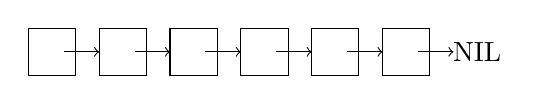
\begin{tikzpicture}[scale=3]
    \foreach \x in {-2, -1.7, ..., -0.4} {
      \draw (\x cm, 1cm) +(-0.1, -0.1) rectangle ++(0.1, 0.1);
      \draw[->] (\x cm, 1cm) +(0.05, 0) -- +(0.2, 0);
    }
    \draw (-0.2cm, 1cm) node {NIL};
    \end{tikzpicture}
  \caption{A list of nodes}
  \label{fig:list-example}
\end{figure}

Every node links to the next one or NIL. Linked-list is often defined through compound structure\footnote{In most cases, the data stored in list have the same type. However, there is also heterogeneous list, like the list in Lisp for example.}, for example:

\lstset{frame=single}
\begin{lstlisting}[language=Bourbaki]
struct List<A> {
    A key
    List<A> next
}
\end{lstlisting}

\index{List!empty} \index{List!empty testing}
It needs more clarification about the empty list. Many traditional environments support {\em null} concept. There are actually two different ways to represent empty list. One is to use null (or NIL) directly; the other is to construct a list, but put nothing as \texttt{[]}. From implementation perspective, null need not allocate any memory, while \texttt{[]} does. In this book, we use $\varnothing$ to represent generic empty list, set, or container.

\subsection{Access}
\index{List!head} \index{List!tail}
\index{List!Construction} \index{List!cons}
Given a list none empty $L$, we need define two functions to access its first element, and the rest sub-list. They are often called $first(L), rest(L)$ or $head(L), tail(L)$\footnote{They are named as \texttt{car} and \texttt{cdr} in Lisp due to the design of machine registers\cite{SICP}.}. On the other hand, we can construct a list from an element $x$ and a sub-list $xs$ (which can be empty), denoted as $x : xs$. It is also called the \texttt{cons} operation. We have the following equations hold:

\be
\begin{cases}
head(x:xs) & = x \\
tail(x:xs) & = xs
\end{cases}
\ee

For a none empty list $X$, we will also use $x_1$ for the first element, and use $X'$ for the rest sub-list. For example, when $X = [x_1, x_2, x_3, ...]$, then $X' = [x_2, x_3, ...]$.

\section{Basic operations}

\index{List!length}
From the list definition, we can count the length recursively: for empty list, the length is zero, otherwise, it is the length of the sub-list plus one.

\be
\begin{array}{rcl}
length(\nil) & = & 0 \\
length(L) & = & 1 + length(L')
\end{array}
\ee

In order to count the length, this algorithm traverses all the elements from the head to the end, hence it is bound to $O(n)$ time, where $n$ is the number of elements in the list. To avoid repeatedly counting, we can also persist the length in a variable, and update it when mutate (add or delete) the list. Below is the iterative way to count the length:

\begin{algorithmic}[1]
\Function{Length}{L}
  \State $n \gets 0$
  \While{$L \neq $ NIL}
    \State $n \gets n + 1$
    \State $L \gets $ \Call{Next}{$L$}
  \EndWhile
  \State \Return $n$
\EndFunction
\end{algorithmic}

We will also use notion $|L|$ for the length of list $L$ when the context is clear.

\subsection{index}
\index{List!index} \index{List!get at}
Different from array, which supports random access an element at position $i$ in constant time, we need traverse the list $i$ steps to access the target element.

\be
getAt(i,\ x:xs) = \begin{cases}
  i = 0: & x \\
  i \neq 0: & getAt(i - 1, xs) \\
\end{cases}
\ee

In order to get the $i$-th element from a none empty list:
\begin{itemize}
\item if $i$ is 0, then we are done, the result is the first element;
\item Otherwise, the result is the $(i-1)$-th element in the sub-list.
\end{itemize}

We intend to leave the empty list not handled. The behavior when pass $\nil$ is undefined. As such the out of bound case also raises undefined error. If $i > |L|$ exceeds the length, we end up the edge case to access the $(i-|L|)$-th element of the empty list. On the other hand, if $i < 0$, minus it by one makes it even farther away from 0. We finally end up with the same undefined error that the index is negative, while the list is empty.

This algorithm is bound to $O(i)$ time as it advances the list $i$ steps. Below is the corresponding imperative implementation:

\begin{algorithmic}[1]
\Function{Get-At}{$i, L$}
  \While{$i \neq 0$}
    \State $L \gets $ \Call{Next}{$L$}  \Comment{Raise error when $L$ = NIL}
    \State $i \gets i - 1$
  \EndWhile
  \State \Return \Call{First}{$L$}
\EndFunction
\end{algorithmic}

\subsection{Last}
\index{List!last} \index{List!init}
There are a pair of symmetric operations to `first/rest'. They are called `last/init'. For a none empty list $X = [x_1, x_2, ..., x_n]$, function $last$ returns the last element $x_1$, while $init$ returns the sub-list of $[x_1, x_2, ..., x_{n-1}]$. Although they are symmetric pairs left to right, `last/init' need linear time, because we need traverse the whole list to tail.


When access the last element of list $X$:
\begin{itemize}
\item If the $X$ contains only one element as $[x_1]$, then $x_1$ is the last one;
\item Otherwise, the result is the last element of the rest sub-list $X'$.
\end{itemize}

\be
\begin{array}{rcl}
last([x]) & = & x \\
last(x:xs) & = & last(xs) \\
\end{array}
\ee

Similarly, when extract the sub-list of $X$ contains all elements without the last one:

\begin{itemize}
\item If $X$ is a singleton $[x_1]$, the result is empty $[\ ]$;
\item Otherwise, we recursively get the initial sub-list for $X'$, then prepend $x_1$ to it as the result.
\end{itemize}

\be
\begin{array}{rcl}
init([x]) & = & [\ ] \\
init(x:xs) & = & x : init(xs) \\
\end{array}
\ee

We leave the empty list not handled for both operations. The behavior is undefined if pass $\nil$ in. Below are the iterative implementation:

\begin{algorithmic}[1]
\Function{Last}{$L$}
  \State $x \gets $ NIL
  \While{$L \neq$ NIL}
    \State $x \gets $ \Call{First}{$L$}
    \State $L \gets $ \Call{Rest}{$L$}
  \EndWhile
  \State \Return $x$
\EndFunction
\Statex
\Function{Init}{$L$}
  \State $L' \gets $ NIL
  \While{\Call{Rest}{$L$} $\neq$ NIL} \Comment{Raise error when $L$ is NIL}
    \State $L' \gets$ \textproc{Cons}(\Call{First}{$L$}, $L'$)
    \State $L \gets $ \Call{Rest}{$L$}
  \EndWhile
  \State \Return \Call{Reverse}{$L'$}
\EndFunction
\end{algorithmic}

As advancing towards the tail, this algorithm accumulates the `init' result through `cons'. However, such result is in the reversed order. We need apply reverse (defined in section \ref{sec:reverse}) again to return the correct result. There is a question to ask if we can use `append' instead of `cons' in the exercise.

\subsection{Reverse index}
\index{List!Reverse index} \index{List!rindex}
Function $last$ is a special case of reverse index. The generic case is to find the last $i$-th element of a given list. The naive implementation takes two rounds of traverse: Determine the length $n$ through the first round; then access the $(n - i - 1)$-th element through the second round:

\be
  lastAt(i, L) = getAt(|L| - i - 1, L)
\ee

There actually exists better solution. The idea is to keep two pointers $p_1, p_2$ with the distance $i$ between them. The equation $rest^i(p_2) = p_1$ holds, where $rest^i(p_2)$ means repleatedly apply $rest()$ function $i$ times. When succeed $p_2$ by $i$ steps gets $p_1$. We start by pointing $p_2$ to the list head, and advance both pointers in parallel till $p_1$ arrives at tail. At that time point, $p_2$ exactly points to the $i$-th element from right. Figure \ref{fig:list-rindex} shows this idea. As $p1, p2$ form a window, this method is also called `sliding window' solution.

\begin{figure}[htbp]
  \centering
  \subcaptionbox{$p_2$ starts from the head, behind $p_1$ in $i$ steps.}{\includegraphics[scale=0.8]{img/list-rindex.ps}} \\
  \subcaptionbox{When $p_1$ reaches the tail, $p_2$ points to the $i$-th element from right.}{\includegraphics[scale=0.8]{img/list-rindex-2.ps}}
  \caption{Sliding window formed by two pointers} \label{fig:list-rindex}
\end{figure}

\begin{algorithmic}[1]
\Function{Last-At}{$i, L$}
  \State $p \gets L$
  \While{$i > 0$}
    \State $L \gets $ \Call{Rest}{$L$} \Comment{Raise error if out of bound}
    \State $i \gets i - 1$
  \EndWhile
  \While{\Call{Rest}{$L$} $\neq$ NIL}
    \State $L \gets$ \Call{Rest}{$L$}
    \State $p \gets$ \Call{Rest}{$p$}
  \EndWhile
  \State \Return \Call{First}{$p$}
\EndFunction
\end{algorithmic}

The functional implementation need special consideration as we cannot update pointers directly. Instead, we advance two lists $X = [x_1, x_2, ..., x_n]$ and $Y = [x_i, x_{i+1}, ..., x_n]$ simultaneously. Where $Y$ is the sub-list without the first $i - 1$ elements.

\begin{itemize}
\item If $Y$ is a singleton list, i.e. $[x_n]$, then the last $i$-th element is the head of $X$;
\item Otherwise, we drop the first element from both $X$ and $Y$, then recursively check $X'$ and $Y'$.
\end{itemize}

\be
lastAt(i, X) = slide(X, drop(i, X))
\ee

where function $slide(X, Y)$ drops the heads element for both lists:

\be
\begin{array}{rcl}
slide(x:xs,\ [y]) & = & x \\
slide(x:xs,\ y:ys) & = & slide(xs, ys) \\
\end{array}
\ee

Function $drop(m, X)$ discard the first $m$ elements from list $X$. It can be implemented by advancing $X$ by $m$ steps:

\be
\begin{array}{rcl}
drop(0,\ X) & = & X \\
drop(m,\ \nil) & = & \nil \\
drop(m,\ x:xs) & = & drop(m - 1, xs) \\
\end{array}
\ee

\subsection{Mutate}
\index{List!mutate}
Mutate operations include append, insert, update, delete elements in a list. Some functional environments actually implement mutate by creating a new list, while the original one is persisted for later reuse, or released at sometime (chapter 2 \cite{okasaki-book}).

\subsubsection{Append}
\index{List!append}
Append is the symmetric operation of $cons$, it add an element on the tail instead of head. Because of this, it is also called `snoc'. For linked-list, it means we need traverse to the tail, hence it takes $O(n)$ time, where $n$ is the length. To avoid repeatedly traverse, we can record the tail reference as a variable, and keep updating it upon changes.

\be
\begin{array}{rcl}
append(\nil, x) & = & [x] \\
append(y:ys, x) & = & y : append(ys, x) \\
\end{array}
\ee

\begin{itemize}
\item If append $x$ to the empty list, the result is $[x]$;
\item Otherwise, we firstly recursive append $x$ to the rest sub-list, then prepend the original head to form the result.
\end{itemize}

The corresponding iterative implementation is as the following:

\begin{algorithmic}[1]
\Function{Append}{$L, x$}
  \If{$L = $ NIL}
    \State \Return \Call{Cons}{$x$, NIL}
  \EndIf
  \State $H \gets L$ \Comment{save the head}
  \While{\Call{Rest}{$L$} $\neq$ NIL}
    \State $L \gets$ \Call{Rest}{$L$}
  \EndWhile
  \State \Call{Rest}{$L$} $\gets$ \Call{Cons}{$x$, NIL}
  \State \Return $H$
\EndFunction
\end{algorithmic}

Update the \textproc{Rest} is typically implemented by setting the \texttt{next} reference field as shown in below example program.

\begin{lstlisting}[language=Bourbaki]
List<A> append(List<A> xs, T x) {
    if (xs == null) {
        return cons(x, null)
    }
    List<A> head = xs
    while (xs.next != null) {
        xs = xs.next
    }
    xs.next = cons(x, null)
    return head
}
\end{lstlisting}

\subsubsection{Set value}
\index{List!set at}
Similar to $getAt$, we need advance to the target position, then change the element there. To define function $setAt(i, x, L)$:

\begin{itemize}
\item If $i = 0$, it means we are changing the first element, the result is $x : L'$;
\item Otherwise, we need recursively set the value at position $i-1$ for the sub-list $L'$.
\end{itemize}

\be
\begin{array}{rcl}
setAt(0, x,\ y:ys) & = & x : ys \\
setAt(i, x,\ y:ys) & = & y : setAt(i - 1, x, ys) \\
\end{array}
\ee

This algorithm is bound to $O(i)$ time, where $i$ is the position to update the value.

\subsubsection{insert}
\index{List!insert} \index{List!insert at}
There are two different cases about insertion. One is to insert an element at a given position: $insert(i, x, L)$. The algorithm is similar to $setAt$; The other is to insert an element to a sorted list, and result is still sorted.

To insert $x$ at position $i$, we need firstly advance $i$ steps, then construct a new sub-list with $x$ as the head, then concatenate it to the first $i$ elements.

\begin{itemize}
\item If $i = 0$, it then turns to be a `cons' operation: $cons(x, L)$;
\item Otherwise, we recursively insert $x$ to $L'$ at position $i-1$; then prepend the original head.
\end{itemize}

\be
\begin{array}{rcl}
insert(0, x,\ L) & = & x : L \\
insert(i, x,\ y:ys) & = & x : insert(i - 1, x, ys) \\
\end{array}
\ee

When $i$ exceeds the length of the list, we can interpret it as to append $x$. We leave this as an exercise. The following is the corresponding iterative implementation:

\begin{algorithmic}[1]
\Function{Insert}{$i, x, L$}
  \If{$i = 0$}
    \State \Return \Call{Cons}{$x, L$}
  \EndIf
  \State $H \gets L$
  \State $p \gets L$
  \While{$i > 0$ and $L \neq$ NIL}
    \State $p \gets L$
    \State $L \gets $ \Call{Rest}{$L$}
    \State $i \gets i - 1$
  \EndWhile
  \State \Call{Rest}{$p$} $\gets$ \Call{Cons}{$x, L$}
  \State \Return $H$
\EndFunction
\end{algorithmic}

If the list $L = [x_1, x_2, ..., x_n]$ is sorted, i.e. for any position $1 \leq i \leq j \leq n$, then $x_i \leq x_j$ holds. Here $\leq$ is abstract as long as the ordering is defined. It can actually means $\geq$ for descending order, or subset relationship etc. We can design the insert algorithm to maintain the sorted order. To insert element $x$ to a sorted list $L$:

\begin{itemize}
\item If either $L$ is empty or $x$ is not greater than the first element in $L$, we prepend $x$ to $L$ and returns $x : L$;
\item Otherwise, we recursively insert $x$ to the sub-list $L'$.
\end{itemize}

\be
\begin{array}{rcl}
insert(x,\ \nil) & = & [x] \\
insert(x,\ y : ys) & = & \begin{cases}
  x \leq y : & x : y : ys \\
  otherwise : & y : insert(x, ys) \\
  \end{cases}
\end{array}
\ee

Since the algorithm need compare elements one by one, it is bound to $O(n)$ time, where $n$ is the length. Below is the corresponding iterative implementation:

\begin{algorithmic}[1]
\Function{Insert}{$x, L$}
  \If{$L = $ NIL or $x <$ \Call{First}{$L$}}
    \State \Return \Call{Cons}{$x, L$}
  \EndIf
  \State $H \gets L$
  \While{\Call{Rest}{$L$} $\neq $ NIL and \textproc{First}(\Call{Rest}{$L$}) $< x$}
    \State $L \gets $ \Call{Rest}{$L$}
  \EndWhile
  \State \Call{Rest}{$L$} $\gets$ \textproc{Cons}($x$, \Call{Rest}{$L$})
  \State \Return $H$
\EndFunction
\end{algorithmic}

\label{sec:isort}
With this linear time ordered insertion defined, we can further develop the insertion-sort algorithm. The idea is to repeatedly insert elements to the empty list. Since each insert takes liner time, the overall sort is bound to $O(n^2)$.

\be
\begin{array}{rcl}
sort(\nil) & = & \nil \\
sort(x:xs) & = & insert(x, sort(xs)) \\
\end{array}
\ee

This is a recursive algorithm. It firstly sorts the sub-list, then inserts the first element in it. We can eliminate the recursion to develop a iterative implementation. The idea is to scan the list, and one by one insert them:

\begin{algorithmic}[1]
\Function{Sort}{$L$}
  \State $L' \gets$ NIL
  \While{$L \neq$ NIL}
    \State $L' \gets$ \textproc{Insert}(\Call{First}{$L$}, $L'$)
    \State $L \gets$ \Call{Rest}{$L$}
  \EndWhile
  \State \Return $L'$
\EndFunction
\end{algorithmic}

At any time during the loop, the result is sorted. There is a major difference between the recursive and the iterative implementations. The recursive one processes the list from right, while the iterative one is from left. We'll introduce `tail-recursion' in section \ref{sec:tail-call} to eliminate this difference. Chapter 3 introduces insertion sort in detail, including performance analysis and optimization.

\subsubsection{delete}
\index{List!delete} \index{List!delete at}
Symmetric to insert, delete also has two cases. One is to delete the element at a position; the other is to look up, then delete the element of a given value. The first case is defined as $delAt(i, L)$, the second case is defined as $delete(x, L)$.

To delete the element at position $i$, we need advance $i$ steps to the target place, then by pass the element, and link the rest sub-list.
\begin{itemize}
\item If $L$ is empty, then the result is empty too;
\item If $i = 0$, that we are deleting the head, the result is $L'$;
\item Otherwise, recursively delete the $(i-1)$-th element from $L'$, then prepend the original head as the result.
\end{itemize}

\be
\begin{array}{rcl}
delAt(i,\ \nil) & = & \nil \\
delAt(0,\ x:xs) & = & xs \\
delAt(i,\ x:xs) & = & x : delAt(i - 1, xs) \\
\end{array}
\ee

This algorithm is bound to $O(i)$ as we need advance $i$ steps to perform deleting. Below is the imperative implementation:

\begin{algorithmic}[1]
\Function{Del-At}{$i, L$}
  \State $S \gets$ \Call{Cons}{$\perp, L$} \Comment{A sentinel node}
  \State $p \gets S$
  \While{$i > 0$ and $L \neq$ NIL}
    \State $i \gets i - 1$
    \State $p \gets L$
    \State $L \gets $ \Call{Rest}{$L$}
  \EndWhile
  \If{$L \neq$ NIL}
    \State \Call{Rest}{$p$} $\gets$ \Call{Rest}{$L$}
  \EndIf
  \State \Return \Call{Rest}{$S$}
\EndFunction
\end{algorithmic}

To simplify the implementation, we introduce a sentinel node $S$, it contains a special value $\perp$, and its next reference points to $L$. With $S$, we are save to cut-off any node in $L$ even for the first one. Finally, we return the list after $S$ as the result, and $S$ itself can be discarded.

For the `find and delete' case, there are two options. We can either find and delete the first occurrence of a value; or remove all the occurrences. The later is more generic, we leave it as an exercise. When delete $x$ from list $L$:

\begin{itemize}
\item If the list is empty, the result is $\nil$;
\item Otherwise, we compare the head and $x$, if they are equal, then the result is $L'$;
\item If the head does not equal to $x$, we keep the head, and recursively delete $x$ in $L'$.
\end{itemize}

\be
\begin{array}{rcl}
delete(x,\ \nil) & = & \nil \\
delete(x,\ y:ys) & = & \begin{cases}
  x = y : & delete(x, ys) \\
  x \neq y : & y : delete(x, ys) \\
  \end{cases} \\
\end{array}
\ee

This algorithm is bound to $O(n)$ time, where $n$ is the length, as it need scan the list to find the target element. For the iterative implementation, we also introduce a sentinel node to simplify the logic:

\begin{algorithmic}[1]
\Function{Delete}{$x, L$}
  \State $S \gets$ \Call{Cons}{$\perp, L$}
  \State $p \gets$ L
  \While{$L \neq$ NIL and \Call{First}{$L$} $\neq x$}
    \State $p \gets L$
    \State $L \gets$ \Call{Rest}{$L$}
  \EndWhile
  \If{$L \neq$ NIL}
    \State \Call{Rest}{$p$} $\gets$ \Call{Rest}{$L$}
  \EndIf
  \State \Return \Call{Rest}{$S$}
\EndFunction
\end{algorithmic}

\subsubsection{concatenate}
\label{concat} \index{List!concat}
Append is a special case for concatenation. Append only adds an element, while concatenation adds multiple ones. However, the performance would be quadratic if repeatedly appending as below:

\be
\begin{array}{rcl}
X \doubleplus \nil & = & X \\
X \doubleplus (y:ys) & = & append(X, y) \doubleplus ys \\
\end{array}
\ee

In this implementation when concatenate $X$ and $Y$, each append operation traverses to the tail, and we do this for $|Y|$ times. the total time is bound to $O(|X| + (|X| + 1) + ... + (|X| + |Y|)) = O(|X||Y| + |Y|^2)$. Consider the link (cons) operation is fast (constant time), we can traverse to the tail of $X$ only once, then link $Y$ to the tail.

\begin{itemize}
\item If $X$ is empty, the result is $Y$;
\item Otherwise, we concatenate the sub-list $X'$ with $Y$, then prepend the head as the result.
\end{itemize}

We can further improve it a bit: when $Y$ is empty, we needn't traverse, but directly return $X$:

\be
\begin{array}{rcl}
\nil \doubleplus Y & = & Y \\
X \doubleplus \nil & = & X \\
(x:xs) \doubleplus Y & = & x : (xs \doubleplus Y) \\
\end{array}
\ee

The modified algorithm only traverse list $X$, then link its tail to $Y$, hence it is bound $O(|X|)$ time. In imperative settings, concatenation can be realized in constant time with the additional tail variable. We leave its implementation as exercise. Below is the iterative implementation without using the tail variable:

\begin{algorithmic}[1]
\Function{Concat}{$X, Y$}
  \If{$X = $ NIL}
    \State \Return $Y$
  \EndIf
  \If{$Y = $ NIL}
    \State \Return $X$
  \EndIf
  \State $H \gets X$
  \While{\Call{Rest}{$X$} $\neq$ NIL}
    \State $X \gets$ \Call{Rest}{$X$}
  \EndWhile
  \State \Call{Rest}{$X$} $\gets Y$
  \State \Return $H$
\EndFunction
\end{algorithmic}

\subsection{sum and product}
\index{List!sum} \index{List!product}
It is common to calculate the sum or product of a list of numbers. They have almost same structure. We will introduce how to abstract them to higher order computation in section \ref{sec:fold}.

\subsubsection{Recursive sum and product}

To calculate the sum of a list:

\begin{itemize}
\item If the list is empty, the result is zero;
\item Otherwise, the result is the first element plus the sum of the rest.
\end{itemize}

\be
\begin{array}{rcl}
sum(\nil) & = & 0 \\
sum(x:xs) & = & x + sum(xs) \\
\end{array}
\ee

We can't merely replace $+$ to $\times$ to obtain product algorithm, because it always returns zero. We need define the product of the empty list as 1.

\be
\begin{array}{rcl}
product(\nil) & = & 1 \\
product(x:xs) & = & x \cdot product(xs) \\
\end{array}
\ee

Both algorithms traverse the list, hence are bound to $O(n)$ time, where $n$ is the length.

\subsubsection{Tail call recursion}
\index{Tail call} \index{Tail recursion} \index{Tail recursive call}
\label{sec:tail-call}
Both sum and product algorithms calculate from right to left. We can change them to calculate the {\em accumulated} result from left to right. For sum, it accumulates from 0, then adds element one by one; while for product, it starts from 1, then repeatedly multiplying elements. The accumulate process can be defined as:

\begin{itemize}
\item If the list is empty, return the accumulated result;
\item Otherwise, accumulate the first element to the result, then and go on accumulating.
\end{itemize}

Below are the accumulated sum and product:

\be
\begin{array}{cc}
  \begin{array}{rl}
  sum'(A,\ \nil) = & A \\
  sum'(A,\ x:xs) = & sum(x + A, xs) \\
  \end{array}
  &
  \begin{array}{rl}
  prod'(A,\ \nil) = & A \\
  prod'(A,\ x:xs) = & prod'(x \cdot A, xs) \\
  \end{array} \\
\end{array}
\ee

Given a list, we can call $sum'$ with 0, and $prod'$ with 1:

\be
sum(X) = sum'(0, X)
\quad \quad \quad
product(X) = prod'(1, X)
\ee

Or merely simplify it to Curried form:

\[
sum = sum'(0) \quad \quad \quad product = prod'(1)
\]

The accumulated sum does not only calculate the result from left to right, it needn't book keeping any context, state, or intermediate result for recursion. All such states are either passed as argument (i.e. $A$), or can be dropped (the previous element in the list). Such recursive calls are often optimized as pure loops in practice. We call this kind of function as {\em tail recursion} (or `tail call'), and the optimization to eliminate recursion is called 'tail recursion optimization'\cite{wiki-tail-call}, because the recursion happens at the tail place in the function. The performance of tail call can be greatly improved after optimization, and we can avoid the issue of stack overflow in deep recursions.

In section \ref{sec:isort} about insertion sort, we mentioned the recursive algorithm sorts elements form right. We can also optimize it to tail call:

\be
\begin{array}{rcl}
sort'(A,\ \nil) & = & A \\
sort'(A,\ x:xs) & = & sort'(insert(x, A), xs) \\
\end{array}
\ee

And the sort is defined Curried form with $\nil$ as the start value:

\be
sort = sort'(\nil)
\ee

As a typical tail call problem, let's consider how to compute $b^n$ effectively? (refer to problem 1.16 in \cite{SICP}.) A brute-force solution is to repeatedly multiplying $b$ for $n$ times from 1. This algorithm is bound to $O(n)$:

\begin{algorithmic}[1]
\Function{Pow}{$b, n$}
  \State $x \gets 1$
  \Loop{ $n$ times}
    \State $x \gets x b$
  \EndLoop
  \State \Return $x$
\EndFunction
\end{algorithmic}

Actually, the solution can be greatly improved. When compute $b^8$, after the first 2 loops, we get $x = b^2$. At this stage, we
needn't multiply $x$ with $b$ to get $b^3$, but directly compute $x^2$, which gives $b^4$. If do this again, we get $(b^4)^2 = b^8$. Thus we only need loop 3 times, but not 8 times.

Based on this idea, if $n = 2^m$ for some none negative integer $m$, we can design below algorithm to compute $b^n$:

\[
\begin{array}{rcl}
b^1 & = & b \\
b^n & = & (b^{\frac{n}{2}})^2 \\
\end{array}
\]

We next extend this divide and conquer method for any none negative integer $n$:

\begin{itemize}
\item If $n = 0$, define $b^0 = 1$;
\item If $n$ is even, we halve $n$, to compute $b^{\frac{n}{2}}$. Then square it;
\item Otherwise $n$ is odd. Since $n-1$ is even, we recursively compute $b^{n-1}$, the multiply $b$ atop it.
\end{itemize}

\be
\begin{array}{rcl}
b^0 & = & 1 \\
b^n & = & \begin{cases}
2 | n : & (b^{\frac{n}{2}})^2 \\
otherwise : & b \cdot b^{n-1} \\
\end{cases}
\end{array}
\ee

However, the 2nd clause blocks us to turn it tail recursive.Alternatively, we can square the base number, and halve the exponent.

\be
\begin{array}{rcl}
b^0 & = & 1 \\
b^n & = & \begin{cases}
2 | n : & (b^2)^{\frac{n}{2}} \\
otherwise : & b \cdot b^{n-1} \\
\end{cases}
\end{array}
\ee

With this change, we can develop a tail recursive algorithm to compute $b^n = pow(b, n, 1)$.

\be
\begin{array}{rcl}
pow(b, 0, A) & = & A \\
pow(b, n, A) & = & \begin{cases}
  2 | n : & pow(b^2, \dfrac{n}{2}, A) \\
  otherwise: & pow(b, n - 1, b \cdot A) \\
\end{cases}
\end{array}
\ee

Compare to the brute-force implementation, this one improves to $O(\lg n)$ time. Actually, we can improve it further. If represent $n$ in binary format $n = (a_ma_{m-1}...a_1a_0)_2$, we clear know
that the computation for $b^{2^i}$ is necessary if $a_i = 1$. This is quite similar to the idea of Binomial heap (section \autoref{sec:binomial-heap}). We can multiplying all of them for bits of 1.

For example, when compute $b^{11}$, as $11 = (1011)_2 = 2^3 + 2 +1$, thus $b^{11} = b^{2^3} \times b^2 \times b$. We get the result by these steps:

\begin{enumerate}
\item calculate $b^1$, which is $b$;
\item Square to $b^2$ from the previous result;
\item Square again to $b^{2^2}$ from step 2;
\item Square to $b^{2^3}$ from step 3.
\end{enumerate}

Finally, we multiply the result of step 1, 2, and 4 to get $b^{11}$. Summarize this idea, we improve the algorithm as below.

\be
\begin{array}{rcl}
pow(b, 0, A) & = & A \\
pow(b, n, A) & = & \begin{cases}
  2 | n : & pow(b^2, \dfrac{n}{2}, A) \\
  otherwise: & pow(b^2, \lfloor \dfrac{n}{2} \rfloor, b \cdot A) \\
  \end{cases}
\end{array}
\ee

This algorithm essentially shifts $n$ to right 1 bit each time (divide $n$ by 2). If the LSB (Least Significant Bit, the lowest) is 0, $n$ is even. It squares the base and keeps the accumulator $A$ unchanged; If the LSB is 1, $n$ is odd. It squares the base and accumulates it to $A$; When $n$ is zero, we exhaust all bits in $n$, $A$ is the final result. At any time, the updated base number $b'$, the shifted exponent number $n'$, and the accumulator $A$ satisfy the invariant $b^n = A \cdot (b')^{n'}$.

Compare to previous one, which minus by one for odd $n$, this algorithm halves $n$ every time. It exactly runs $m$ rounds, where $m$ is the number of bits. We leave the imperative implementation as exercise.

Back to the sum and product operations. The iterative implementation applies plus and multiplication while traverse the list:

\begin{algorithmic}[1]
\Function{Sum}{$L$}
  \State $s \gets 0$
  \While{$L \neq$ NIL}
    \State $s \gets s +$ \Call{First}{$L$}
    \State $L \gets$ \Call{Rest}{$L$}
  \EndWhile
  \State \Return $s$
\EndFunction
\Statex
\Function{Product}{$L$}
  \State $p \gets 1$
  \While{$L \neq$ NIL}
    \State $p \gets p \times $ \Call{First}{$L$}
    \State $L \gets$ \Call{Rest}{$L$}
  \EndWhile
  \State \Return $p$
\EndFunction
\end{algorithmic}

One interesting usage of product is to calculate factorial of $n$ as: $n! = product([1..n])$.

\subsection{maximum and minimum}
\index{List!maximum} \index{List!minimum}

For a list of comparable elements (we can define order for any two elements), there is the maximum and minimum. The algorithm structure of $max/min$ is same. For a none empty list:

\begin{itemize}
\item If there is only one element (a singleton) $[x_1]$, the result is $x_1$;
\item Otherwise, we recursively find the min/max of the sub-list, then compare it with the first element to determine the result.
\end{itemize}

\be
  \begin{array}{rcl}
  min([x]) & = & x \\
  min(x:xs) & = & \begin{cases}
    x < min(xs) : & x \\
    otherwise: & min(xs) \\
  \end{cases}
  \end{array}
\ee
and
\be
  \begin{array}{rcl}
  max([x]) & = & x \\
  max(x:xs) & = & \begin{cases}
    x > max(xs) : & x \\
    otherwise: & max(xs) \\
  \end{cases}
  \end{array}
\ee

Both process the list from right to left. We can modify them to tail recursive form. It also brings us the `on-line' feature, that at any time, the accumulator is the min/max so far processed. Use $min$ for example:

\be
\begin{array}{rcl}
min'(a,\ \nil) & = & a \\
min'(a,\ x:xs) & = & \begin{cases}
  x < a : & min'(x, xs) \\
  otherwise : & min'(a, xs) \\
  \end{cases}
\end{array}
\ee

Different from $sum'/prod'$, we can't pass a fixed starting value to the tail recursive $min'/max'$, unless we use $\pm \infty$ in below Curried form:

\[
  min = min'(\infty) \quad \quad \quad max = max'(- \infty)
\]

Alternatively, we can pass the first element as the accumulator give min/max only take none empty list:

\be
  min(x:xs) = min'(x,\ xs)
  \quad \quad \quad
  max(x:xs) = max'(x,\ xs)
\ee

The optimized tail recursive algorithm can be further changed to purely iterative implementation. We give \textproc{Min} example, and skip \textproc{Max}.

\begin{algorithmic}[1]
\Function{Min}{$L$}
  \State $m \gets$ \Call{First}{$L$}
  \State $L \gets$ \Call{Rest}{$L$}
  \While{$L \neq$ NIL}
    \If{\Call{First}{$L$} $< m$ }
      \State $m \gets$ \Call{First}{$L$}
    \EndIf
    \State $L \gets$ \Call{Rest}{$L$}
  \EndWhile
  \State \Return $m$
\EndFunction
\end{algorithmic}

There is a way to realize the tail recursive algorithm without using accumulator explicitly. The idea is to re-use the first element as the accumulator. Every time, we compare the head with the next one; then drop the greater for $min$, and drop the less for $max$.

\be
\begin{array}{rcl}
min([x]) & = & x \\
min(x_1:x_2:xs) & = & \begin{cases}
  x_1 < x_2 : & min(x_1:xs) \\
  otherwise: & min(x_2:xs) \\
  \end{cases}
\end{array}
\ee

We skip the definition for $max$ as it is symmetric.

\begin{Exercise}
\Question{For list of type $A$, suppose we can test if any two elements $x, y \in A$ are equal, define an algorithm to test if two lists are identical to each other.}
\Question{In the \textproc{Get-At}($i, L$) algorithm, what is the behavior when $L$ is empty? what is the behavior when $i$ is out of the bound or negative?}
\Question{In the \textproc{Init} algorithm, can we use \textproc{Append}($L'$, \textproc{First}($L$)) instead of `cons'?}
\Question{How to handle empty list or out of bound index error in \textproc{Last-At} algorithm?}
\Question{Add a `tail' field in list definition, optimize the append algorithm to constant time.}
\Question{With the additional `tail' field, when we need update the tail variable? How does it affect the performance?}
\Question{Handle the empty list and out of bound error for $setAt$.}
\Question{Handle the out-of-bound case in insertion, and treat it as append.}
\Question{Implement the insertion sort only with less than ($<$) defined.}
\Question{Develop the algorithm to find and delete all occurrences of a given value.}
\Question{Change the $length$ to tail call.}
\Question{Change the insertion sort to tail call.}
\Question{Implement the $O(\lg n)$ algorithm to calculate $b^n$ by represent $n$ in binary.}
\end{Exercise}

\section{Transform}
\index{List!Transform}
From algebraic perspective, there are two types of transform: one keeps the list structure, but only change the elements; the other alter the list structure, hence the result is not isomorphic to the original list. Particularly, we call the former map.

\subsection{map and for-each}
\index{List!map}
The first example is to convert a list of number to their represented strings, like to change [3, 1, 2, 4, 5] to [``three'', ``one'', ``two'', ``four'', ``five'']

\be
\begin{array}{rcl}
toStr(\nil) & = & \nil \\
toStr(x:xs) & = & str(x) : toStr(xs) \\
\begin{array}
\label{eq:tostr}
\ee

For the second example, consider a dictionary, which is a list of words grouped by initial letter. Like:

\begin{verbatim}
[[a, an, another, ... ],
 [bat, bath, bool, bus, ...],
 ...,
 [zero, zoo, ...]]
\end{verbatim}

Next we process a text ({\em Hamlet} for example), and augment each word with their number of occurrence, like:

\begin{verbatim}
[[(a, 1041), (an, 432), (another, 802), ... ],
 [(bat, 5), (bath, 34), (bool, 11), (bus, 0), ...],
 ...,
 [(zero 12), (zoo, 0), ...]]
\end{verbatim}

Now for every initial letter, we want to figure out which word occurs most. How to write a program to do this work? The output is a list of words, that every one has the most occurrences in the group, something like \texttt{[a, but, can, ...]}. We need develop a program that transform \textbf{a list of groups of word-number pairs} into \textbf{a list of words}.

Let's work it out step by step. First, we need define a function, which takes a list of word - number pairs, and find the
word has the biggest number augmented. Sorting is overkill. What we need is just a special $max'()$ function, Note that the
$max()$ function developed in previous section can't be used directly. Suppose for a pair of values $p = (a, b)$, function
$fst(p) = a$, and $snd(p) = b$ are accessors to extract the values, $max'()$ can be defined as the following.

\be
max'(L) = \left \{
  \begin{array}
  {r@{\quad:\quad}l}
  l_1 & |L| = 1 \\
  l_1 & snd(max'(L')) < snd(l_1) \\
  max'(L') & otherwise
  \end{array}
\right.
\ee

Alternatively, we can define a dedicated function to compare word-number of occurrence pair, and generalize the
$max()$ function by passing a compare function.

\be
less(p_1, p_2) = snd(p_1) < snd(p_2)
\ee

\be
maxBy(cmp, L) = \left \{
  \begin{array}
  {r@{\quad:\quad}l}
  l_1 & |L| = 1 \\
  l_1 & cmp(l_1, maxBy(cmp, L')) \\
  maxBy(cmp, L') & otherwise
  \end{array}
\right.
\ee

Then $max'()$ is just a special case of $maxBy()$ with the compare function comparing on the second value in a pair.

\be
max'(L) = maxBy(\neg less, L)
\ee

Here we write all functions in purely recursive way, they can be modified in tail call manner. This is left as exercise
to the reader.

With $max'()$ function defined, it's possible to complete the solution by processing the whole list.

\be
solve(L) = \left \{
  \begin{array}
  {r@{\quad:\quad}l}
  \phi & L = \phi \\
  cons(fst(max'(l_1)), solve(L')) & otherwise
  \end{array}
\right.
\label{eq:solve}
\ee

\subsubsection{Map}
\index{List!map}

Compare the $solve()$ function in (\ref{eq:solve}) and $toStr()$ function in (\ref{eq:tostr}), it reveals very similar
algorithm structure. although they targets on very different problems, and one is trivial while the other is a bit
complex.

The structure of $toStr()$ applies the function $str()$ which can turn a number into string on every element in the list;
while $solve()$ first applies $max'()$ function to every element (which is actually a list of pairs), then applies $fst()$
function, which essentially turns a list of pairs into a string. It is not hard to abstract such common structure like
the following equation, which is called as {\em mapping}.

\be
map(f, L) =  \left \{
  \begin{array}
  {r@{\quad:\quad}l}
  \phi & L = \phi \\
  cons(f(l_1)), map(f, L')) & otherwise
  \end{array}
\right.
\ee

Because map takes a `converter' function $f$ as argument, it's called a kind of high-order function. In functional
programming environment such as Haskell, mapping can be implemented just like the above equation.

\lstset{language=Haskell}
\begin{lstlisting}
map :: (a->b)->[a]->[b]
map _ [] = []
map f (x:xs) = f x : map f xs
\end{lstlisting}

The two concrete cases we discussed above can all be represented in high order mapping.

\[
\begin{array}{l}
toStr  = map \quad str \\
solve = map \quad (fst \cdot max')
\end{array}
\]

Where $f \cdot g$ means function composing, that we first apply $g$ then apply $f$. For instance
function $h(x) = f(g(x))$ can be represented as $h = f \cdot g $, reading like function $h$ is
composed by $f$ and $g$. Note that we use Curried form to omit the argument $L$ for brevity.
Informally speaking, If we feed a function which needs 2 arguments, for instance $f(x, y) = z$
with only 1 argument, the result turns to be a function which need 1 argument. For instance,
if we feed $f$ with only argument $x$, it turns to be a new function take one argument $y$,
defined as $g(y) = f(x, y)$, or $g = f x$. Note that $x$ isn't a free variable any more,
as it is bound to a value. Reader can refer to any book about functional programming
for details about function composing and Currying.

Mapping can also be understood from the domain theory point of view. Consider function $y = f(x)$,
it actually defines a mapping from domain of variable $x$ to the domain of value $y$. ($x$
and $y$ can have different types). If the domains can be represented as set $X$, and $Y$, we have
the following relation.

\be
Y = \{ f(x) | x \in X \}
\ee

This type of set definition is called Zermelo Frankel set abstraction (as known as ZF expression) \cite{algo-fp}. The different
is that here the mapping is from a list to another list, so there can be duplicated elements.
In languages support list comprehension, for example Haskell and Python etc (Note that the
Python list is a built-in type, but not the linked-list we discussed in this appendix), mapping
can be implemented as a special case of list comprehension.

\lstset{language=Haskell}
\begin{lstlisting}
map f xs = [ f x | x <- xs]
\end{lstlisting}

List comprehension is a powerful tool. Here is another example that realizes the permutation
algorithm in list comprehension. Many textbooks introduce how to implement all-permutation
for a list, such as \cite{algo-fp}, and \cite{erlang}. It is possible to design a more general
version $perm(L, r)$, that if the length of the list $L$ is $n$, this algorithm permutes
$r$ elements from the total $n$ elements. We know that there are $P_n^r = \frac{n!}{(n-r)!}$
solutions.

\be
perm(L, r) = \left \{
  \begin{array}
  {r@{\quad:\quad}l}
  \{\phi\} & r = 0 \lor |L| < r \\
  \{ \{l\} \cup P | l \in L, P \in perm(L-\{l\}, r-1)\} & otherwise
  \end{array}
\right.
\ee

In this equation, $\{l\} \cup P$ means $cons(l, P)$, and $L-\{l\}$ denotes $delete(L, l)$, which
is defined in previous section. If we take zero element for permutation, or there are too
few elements (less than $r$), the result is a list contains a empty list; Otherwise for non-trivial
case, the algorithm picks one element $l$ from the list, and recursively permutes the rest $n-1$
elements by picking up $r-1$ ones; then it puts all the possible $l$ in front of all the possible
$r-1$ permutations. Here is the Haskell implementation of this algorithm.

\lstset{language=Haskell}
\begin{lstlisting}
perm _ 0 = [[]]
perm xs r | length xs < r = [[]]
          | otherwise = [ x:ys | x <-xs, ys <- perm (delete x xs) (r-1)]
\end{lstlisting}

We'll go back to the list comprehension later in section about filtering.

Mapping can also be realized imperatively. We can apply the
function while traversing the list, and construct the new list from left to right.
Since that the new element is appended to the result list, we can track the tail
position to achieve constant time appending, so the mapping algorithms is linear in
terms of the passed in function.

\begin{algorithmic}[1]
\Function{Map}{$f, L$}
  \State $L' \gets \phi$
  \State $p \gets \phi$
  \While{$L \neq \phi$}
    \If{$p = \phi$}
      \State $p \gets$ \textproc{Cons}($f($ \Call{First}{$L$} $), \phi$)
      \State $L' \gets p$
    \Else
      \State \Call{Next}{$p$} $\gets$ \textproc{Cons}($f($ \Call{First}{$L$} $), \phi$)
      \State $p \gets$ \Call{Next}{$p$}
    \EndIf
    \State $L \gets$ \Call{Next}{$L$}
  \EndWhile
  \State \Return $L'$
\EndFunction
\end{algorithmic}

In some static typed programming luangaes without type inference feature, like C++\footnote{At least in ISO C++ 1998 standard.}, It is a bit complex to annotate the type of the passed-in function. See \cite{sgi-stl-transform} for detail.
In fact some C++ environment provides the very same mapping concept as in \texttt{std::transform}. However,
it needs the reader to know some language specific features, which are out of the scope of this book.

For brevity purpose, we switch to Python programming language for example code. So that the type inference
can be avoid in compile time. The definition of a simple singly linked-list in Python is give as the
following.

\lstset{language=Python}
\begin{lstlisting}
class List:
    def __init__(self, x = None, xs = None):
        self.key = x
        self.next = xs

def cons(x, xs):
    return List(x, xs)
\end{lstlisting}

The mapping program, takes a function and a linked-list, and maps the functions to every element as described
in above algorithm.

\begin{lstlisting}
def mapL(f, xs):
    ys = prev = List()
    while xs is not None:
        prev.next = List(f(xs.key))
        prev = prev.next
        xs = xs.next
    return ys.next
\end{lstlisting}

Different from the pseudo code, this program uses a dummy node as the head of the resulting list. So it needn't
test if the variable stores the last appending position is NIL. This small trick makes the program compact.
We only need drop the dummy node before returning the result.

\subsubsection{For each}
\index{List!for each}

For the trivial task such as printing a list of elements out, it's quite OK to just print each element without
converting the whole list to a list of strings. We can actually simplify the program.

\begin{algorithmic}[1]
\Function{Print}{$L$}
  \While{$L \neq \phi$}
    \State print \Call{First}{$L$}
    \State $L \gets$ \Call{Rest}{$L$}
  \EndWhile
\EndFunction
\end{algorithmic}

More generally, we can pass a procedure such as printing, to this list traverse, so the procedure is
performed {\em for each} element.

\begin{algorithmic}[1]
\Function{For-Each}{$L, P$}
  \While{$L \neq \phi$}
    \State \textproc{P}(\Call{First}{$L$})
    \State $L \gets$ \Call{Rest}{$L$}
  \EndWhile
\EndFunction
\end{algorithmic}

For-each algorithm can be formalized in recursive approach as well.

\be
foreach(L, p) = \left \{
  \begin{array}
  {r@{\quad:\quad}l}
  u & L = \phi \\
  do(p(l_1), foreach(L', p)) & otherwise
  \end{array}
\right.
\ee

Here $u$ means unit, it's can be understood as doing nothing. The type of unit is similar to the `void' concept
in C or java like programming languages. The $do()$ function evaluates all its arguments, discards all
the results except for the last one, and returns the last result as the final value of $do()$. It is
equivalent to \texttt{(begin ...)} in Lisp families, and \texttt{do} block in Haskell in some sense.
For the details about unit type, please refer to \cite{mittype}.

Note that the for-each algorithm is just a simplified mapping, there are only two minor difference points:

\begin{itemize}
\item It needn't form a result list, we care the `side effect' rather than the returned value;
\item For each focus more on traversing, while mapping focus more on applying function, thus the order
of arguments are typically arranged as $map(f, L)$ and $foreach(L, p)$.
\end{itemize}

Some Functional programming facilities provide options for both returning the result list or discarding it.
For example Haskell Monad library provides both \texttt{mapM}, \texttt{mapM\_} and \texttt{forM}, \texttt{forM\_}.
Readers can refer to language specific materials for detail.

\subsubsection{Examples for mapping}

We'll show how to use mapping by an example, which is a problem of ACM/ICPC\cite{poj-drunk-jailer}.
For sake of brevity, we modified the problem description a bit. Suppose there are $n$ lights in a room, all
of them are off. We execute the following process $n$ times:

\begin{enumerate}
\item We switch all the lights in the room, so that they are all on;
\item We switch the 2, 4, 6, ... lights, that every other light is switched, if the light is on, it will be off, and it will be
on if the previous state is off;
\item We switch every third lights, that the 3, 6, 9, ... are switched;
\item ...
\end{enumerate}

And at the last round, only the last light (the $n$-th light) is switched.

The question is how many lights are on finally?

Before we show the best answer to this puzzle, let's first work out a naive brute-force solution.
Suppose there are $n$ lights, which can be represented as a list of 0, 1 numbers, where 0 means the light
is off, and 1 means on. The initial state is a list of $n$ zeros: $\{0, 0, ..., 0\}$.

We can label the light from 1 to $n$. A mapping can help us to turn the above list into a labeled list\footnote{Readers
who are familiar with functional programming, may use zipping to achieve this. We'll explain zipping in later
section.}.

\[
map(\lambda_i \cdot (i, 0), \{1, 2, 3, ... n\})
\]

This mapping augments each natural number with zero, the result is a list of pairs: $L = \{(1, 0), (2, 0), ..., (n, 0)\}$.

Next we operate this list of pairs $n$ times from 1 to $n$. For every time $i$, we switch the second value in this pair
if the first label can be divided by $i$. Consider the fact that $1 - 0 = 1$, and $1 - 1 = 0$, we can realize switching
of 0, 1 value $x$ by $1 - x$. At the $i$-th operation, for light $(j, x)$, if $i | j$, (or $j \mod i = 0$), we then
perform switching, otherwise, we leave the light untouched.

\be
switch(i, (j, x)) = \left \{
  \begin{array}
  {r@{\quad:\quad}l}
  (j, 1 - x) &  j \mod i = 0 \\
  (j, x) & otherwise
  \end{array}
\right.
\ee

The $i$-th operation on all lights can be realized as mapping again:

\be
map(switch(i), L)
\ee

Note that, here we use Curried form of $switch()$ function, which is equivalent to

\[
map(\lambda_{(j, x)} \cdot switch(i, (j, x)), L)
\]

Here we need define a function $proc()$, which can perform the above mapping on $L$ over and over by $n$ times.
One option is to realize it in purely recursive way as the following, so that we can call it like
$proc(\{1, 2, ..., n\}, L)$\footnote{This can also be realized by folding, which will be explained in later section.}.

\be
proc(I, L) = \left \{
  \begin{array}
  {r@{\quad:\quad}l}
  L & I = \phi \\
  operate(I', map(switch(i_1), L)) & otherwise
  \end{array}
\right.
\ee

Where $I = cons(i_1, I')$ if $I$ isn't empty.

At this stage, we can sum the second value of each pair in list $L$ to get the answer. The sum function has been
defined in previous section, so the only thing left is mapping.

\be
solve(n) = sum(map(snd, proc(\{1, 2, ..., n\}, L)))
\ee

Translating this naive brute-force solution to Haskell yields below program.

\lstset{language=Haskell}
\begin{lstlisting}
solve' = sum . (map snd) . proc  where
    proc n = operate [1..n] $ map (\i -> (i, 0)) [1..n]
    operate [] xs = xs
    operate (i:is) xs = operate is (map (switch i) xs)

switch i (j, x) = if j `mod` i == 0 then (j, 1 - x) else (j, x)
\end{lstlisting} %$

Let's see what's the answer for there are 1, 2, ..., 100 lights.

\begin{verbatim}
[1,1,1,2,2,2,2,2,3,3,3,3,3,3,3,4,4,4,4,4,4,4,4,4,5,5,5,5,5,5,5,5,5,5,5,
6,6,6,6,6,6,6,6,6,6,6,6,6,7,7,7,7,7,7,7,7,7,7,7,7,7,7,7,8,8,8,8,8,8,8,
8,8,8,8,8,8,8,8,8,8,9,9,9,9,9,9,9,9,9,9,9,9,9,9,9,9,9,9,9,10]
\end{verbatim}

This result is interesting:

\begin{itemize}
\item the first 3 answers are 1;
\item the 4-th to the 8-th answers are 2;
\item the 9-th to the 15-th answers are 3;
\item ...
\end{itemize}

It seems that the $i^2$-th to the $((i+1)^2-1)$-th answers are $i$. Actually, we can prove this fact as the following.

\begin{proof}
Given $n$ lights, labeled from 1 to $n$, consider which lights are on finally. Since the initial states for all lights
are off, we can say that, the lights which are manipulated odd times are on. For every light $i$, it will be switched
at the $j$ round if $i$ can be divided by $j$ (denote as $j | i$). So only the lights which have odd number of factors are on at the end.

So the key point to solve this puzzle, is to find all numbers which have odd number of factors. For any positive integer
$n$, denote $S$ the set of all factors of $n$. $S$ is initialized to $\phi$. if $p$ is a factor of $n$, there must
exist a positive integer $q$ that $n = p q$, which means $q$ is also a factor of $n$. So we add 2 different factors to
the set $S$ if and only if $p \neq q$, which keeps $|S|$ even all the time unless $p = q$. In such case, $n$ is a
perfect square number, and we can only add 1 factor to the set $S$, which leads to an odd number of factors.
\end{proof}


At this stage, we can design a fast solution by finding the number of perfect square numbers under $n$.

\be
solve(n) = \lfloor \sqrt{n} \rfloor
\ee

The next Haskell command verifies that the answer for 1, 2, ..., 100 lights are as same as above.

\begin{lstlisting}
map (floor.sqrt) [1..100]
[1,1,1,2,2,2,2,2,3,3,3,3,3,3,3,4,4,4,4,4,4,4,4,4,5,5,5,5,5,5,5,5,5,5,5,
6,6,6,6,6,6,6,6,6,6,6,6,6,7,7,7,7,7,7,7,7,7,7,7,7,7,7,7,8,8,8,8,8,8,8,
8,8,8,8,8,8,8,8,8,8,9,9,9,9,9,9,9,9,9,9,9,9,9,9,9,9,9,9,9,10]
\end{lstlisting}

Mapping is generic concept that it doesn't only limit in linked-list, but also can be applied to many
complex data structures. The chapter about binary search tree in this book explains how to map on trees.
As long as we can traverse a data structure in some order, and the empty data structure can be identified,
we can use the same mapping idea. We'll return to this kind of high-order concept in the section of folding
later.

\subsection{reverse}
\index{List!reverse} \label{sec:reverse}
How to reverse a singly linked-list with minimum space is a popular technical interview problem in some companies.
The pointer manipulation must be arranged carefully in imperative programming languages such as ANSI C.
However, we'll show that, there exists an easy way to write this program:

\begin{enumerate}
\item Firstly, write a pure recursive straightforward solution;
\item Then, transform the pure recursive solution to tail-call manner;
\item Finally, translate the tail-call solution to pure imperative pointer operations.
\end{enumerate}

The pure recursive solution is simple enough that we can write it out immediately. In order to {\em reverse a list} $L$.

\begin{itemize}
\item If $L$ is empty, the reversed result is empty. This is the trivial edge case;
\item Otherwise, we can first reverse the rest of the sub-list, then append the first element to the end.
\end{itemize}

This idea can be formalized to the below equation.

\be
reverse(L) =  \left \{
  \begin{array}
  {r@{\quad:\quad}l}
  \phi & L = \phi \\
  append(reverse(L'), l_1) & otherwise \\
  \end{array}
\right.
\ee

Translating it to Haskell yields below program.

\lstset{language=Haskell}
\begin{lstlisting}
reverse [] = []
reverse (x:xs) = reverse xs ++ [x]
\end{lstlisting}

However, this solution doesn't perform well, as appending has to traverse to the end of list, which leads to a quadratic time
algorithm. It is not hard to improve this program by changing it to tail-call manner. That we can use a accumulator to store
the intermediate reversed result, and initialize the accumulated result as empty. So the algorithm is formalized as
$reverse(L) = reverse'(L, \phi)$.

\be
reverse'(L, A) =  \left \{
  \begin{array}
  {r@{\quad:\quad}l}
  A & L = \phi \\
  reverse'(L', \{l_1\} \cup A) & otherwise
  \end{array}
\right.
\ee

Where $\{l_1\} \cup A$ means $cons(l_1, A)$. Different from appending, it's a constant $O(1)$ time operation. The core idea is
that we repeatedly take the element one by one from the head of the original list, and put them in front the accumulated
result. This is just like we store all the elements in a stack, them pop them out. This is a linear time algorithm.

Below Haskell program implements this tail-call version.

\begin{lstlisting}
reverse' [] acc = acc
reverse' (x:xs) acc = reverse' xs (x:acc)
\end{lstlisting}

Since the nature of tail-recursion call needn't book-keep any context (typically by stack), most modern compilers are
able to optimize it to a pure imperative loop, and reuse the current context and stack etc. Let's manually do this
optimization so that we can get a imperative algorithm.

\begin{algorithmic}[1]
\Function{Reverse}{$L$}
  \State $A \gets \phi$
  \While{$L \neq \phi$}
    \State $A \gets $ \textproc{Cons}(\Call{First}{$L$}, $A$)
    \State $L \gets$ \Call{Rest}{$L$}
  \EndWhile
\EndFunction
\end{algorithmic}

However, because we translate it directly from a functional solution, this algorithm actually produces a new reversed list,
but does not mutate the original one. It is not hard to change it to an in-place solution by reusing $L$. For example, the following
ISO C++ program implements the in-place algorithm. It takes $O(1)$ memory space, and reverses the list in $O(n)$ time.

\lstset{language=C++}
\begin{lstlisting}
template<typename T>
List<T>* reverse(List<T>* xs) {
  List<T> *p, *ys = NULL;
  while (xs) {
    p = xs;
    xs = xs->next;
    p->next = ys;
    ys = p;
  }
  return ys;
}
\end{lstlisting}

\begin{Exercise}
\begin{itemize}
\item Implement the algorithm to find the maximum element in a list of pair in tail call approach in your favorite programming
language.
\end{itemize}
\end{Exercise}

\section{Extract sub-lists}
\index{List!Extract sub-list}
Different from arrays which are capable to slice a continuous segment fast and easily, It needs more work to extract sub lists
from singly linked list. Such operations are typically linear algorithms.

\subsection{take, drop, and split-at}
\index{List!take}
\index{List!drop}
\index{List!split at}

Taking first $n$ elements from a list is semantically similar to extract sub list from the very left like $sublist(L, 1, n)$,
where the second and the third arguments to $sublist$ are the positions the sub-list starts and ends.
For the trivial edge case, that either $n$ is zero or the list is empty, the sub list is empty; Otherwise, we
can recursively take the first $n-1$ elements from the rest of the list, and put the first element in front of it.

\be
take(n, L) = \left \{
  \begin{array}
  {r@{\quad:\quad}l}
  \phi & L = \phi \lor n = 0 \\
  cons(l_1, take(n-1, L')) & otherwise
  \end{array}
\right.
\ee

Note that the edge cases actually handle the out-of-bound error. The following Haskell program implements this algorithm.

\lstset{language=Haskell}
\begin{lstlisting}
take _ [] = []
take 0 _ = []
take n (x:xs) = x : take (n-1) xs
\end{lstlisting}

Dropping on the other hand, drops the first $n$ elements and returns the left as result. It is equivalent to get the
sub list from right like $sublist(L, n+1, |L|)$, where $|L|$ is the length of the list. Dropping can be designed quite similar
to taking by discarding the first element in the recursive case.

\be
drop(n, L) = \left \{
  \begin{array}
  {r@{\quad:\quad}l}
  \phi & L = \phi \\
  L & n = 0 \\
  drop(n-1, L')) & otherwise
  \end{array}
\right.
\ee

Translating the algorithm to Haskell gives the below example program.

\lstset{language=Haskell}
\begin{lstlisting}
drop _ [] = []
drop 0 L = L
drop n (x:xs) = drop (n-1) xs
\end{lstlisting}

The imperative taking and dropping are quite straight-forward, that they are left as exercises to the
reader.

With taking and dropping defined, extracting sub list at arbitrary position for arbitrary length can be
realized by calling them.

\be
sublist(L, from, count) = take(count, drop(from - 1, L))
\ee

or in another semantics by providing left and right boundaries:

\be
sublist(L, from, to) = drop(from - 1, take(to, L))
\ee

Note that the elements in range $[from, to]$ is returned by this function, with both ends included.
All the above algorithms perform in linear time.

\subsubsection{take-while and drop-while}
\index{List!take while}
\index{List!drop while}
Compare to taking and dropping, there is another type of operation, that we either keep taking or dropping
elements as far as a certain condition is met. The taking and dropping algorithms can be viewed as special
cases for take-while and drop-while.

Take-while examines elements one by one as far as the condition is satisfied, and ignore all the rest of elements
even some of them satisfy the condition. This is the different point from filtering which we'll explained
in later section. Take-while stops once the condition tests fail; while filtering traverses the whole list.

\be
takeWhile(p, L) =  \left \{
  \begin{array}
  {r@{\quad:\quad}l}
  \phi & L = \phi \\
  \phi & \lnot p(l_1) \\
  cons(l_1, takeWhile(p, L')) & otherwise
  \end{array}
\right.
\ee

Take-while accepts two arguments, one is the predicate function $p$, which can be applied to element in
the list and returns Boolean value as result; the other argument is the list to be processed.

It is easy to define the drop-while symmetrically.

\be
dropWhile(p, L) = \left \{
  \begin{array}
  {r@{\quad:\quad}l}
  \phi & L = \phi \\
  L & \lnot p(l_1) \\
  dropWhile(p, L') & otherwise
  \end{array}
\right.
\ee

The corresponding Haskell example programs are given as below.

\lstset{language=Haskell}
\begin{lstlisting}
takeWhile _ [] = []
takeWhile p (x:xs) = if p x then x : takeWhile p xs else []

dropWhile _ [] = []
dropWhile p xs@(x:xs') = if p x then dropWhile p xs' else xs
\end{lstlisting}

\subsubsection{split-at}
\index{List!split at}
With taking and dropping defined, splitting-at can be realized trivially by calling them.

\be
splitAt(i, L) = (take(i, L), drop(i, L))
\ee

\subsection{breaking and grouping}

\subsubsection{breaking}
\index{List!break}
\index{List!span}

Breaking can be considered as a general form of splitting, instead of splitting at a given position, breaking
examines every element for a certain predicate, and finds the longest prefix of the list for that condition.
The result is a pair of sub-lists, one is that longest prefix, the other is the rest.

There are two different breaking semantics, one is to pick elements satisfying the predicate as long as possible;
the other is to pick those don't satisfy. The former is typically defined as $span$, while the later as $break$.

Span can be described, for example, in such recursive manner: In order to span a list $L$ for predicate $p$:

\begin{itemize}
\item If the list is empty, the result for this edge trivial case is a pair of empty lists $(\phi, \phi)$;
\item Otherwise, we test the predicate against the first element $l_1$, if $l_1$ satisfies the predicate, we
denote the intermediate result for spanning the rest of list as $(A, B) = span(p, L')$, then
 we put $l_1$ in front of $A$ to get pair $(\{ l_1 \} \cup A, B)$, otherwise, we just return $(\phi, L)$ as
the result.
\end{itemize}

For breaking, we just test the negate of predicate and all the others are as same as spanning. Alternatively,
one can define breaking by using span as in the later example program.

\be
span(p, L) =  \left \{
  \begin{array}
  {r@{\quad:\quad}l}
  (\phi, \phi) & L = \phi \\
  (\{ l_1 \} \cup A, B) & p(l_1) = True, (A, B) = span(p, L') \\
  (\phi, L) & otherwise
  \end{array}
\right.
\ee

\be
break(p, L) =  \left \{
  \begin{array}
  {r@{\quad:\quad}l}
  (\phi, \phi) & L = \phi \\
  (\{ l_1 \} \cup A, B) & \lnot p(l_1), (A, B) = break(p, L') \\
  (\phi, L) & otherwise
  \end{array}
\right.
\ee

Note that both functions only find the longest {\em prefix}, they stop immediately when the condition
is fail even if there are elements in the rest of the list meet the predicate (or not). Translating them
to Haskell gives the following example program.

\lstset{language=Haskell}
\begin{lstlisting}
span _ [] = ([], [])
span p xs@(x:xs') = if p x then let (as, bs) = span p xs' in (x:as, bs) else ([], xs)

break p = span (not . p)
\end{lstlisting}

Span and break can also be realized imperatively as the following.

\begin{algorithmic}[1]
\Function{Span}{$p, L$}
  \State $A \gets \phi$
  \While{$L \neq \phi \land p(l_1)$}
    \State $A \gets $ \Call{Cons}{$l_1, A$}
    \State $L \gets $ \Call{Rest}{$L$}
  \EndWhile
  \State \Return $(A, L)$
\EndFunction
\Statex
\Function{Break}{$p, L$}
  \State \Return \Call{Span}{$\lnot p, L$}
\EndFunction
\end{algorithmic}

This algorithm creates a new list to hold the longest prefix, another option is to turn it
into in-place algorithm to reuse the spaces as in the following Python example.

\lstset{language=Python}
\begin{lstlisting}
def span(p, xs):
    ys = xs
    last = None
    while xs is not None and p(xs.key):
        last = xs
        xs = xs.next
    if last is None:
        return (None, xs)
    last.next = None
    return (ys, xs)
\end{lstlisting}

Note that both span and break need traverse the list to test the predicate, thus they are linear
algorithms bound to $O(n)$.

\subsubsection{grouping}
\index{List!group}
Grouping is a commonly used operation to solve the problems that we need divide the list into some small groups.
For example, Suppose we want to group the
string `Mississippi', which is actual a list of char \{ 'M', 's', 's', 'i', 's', 's', 'i', 'p', 'p', 'i'\}.
into several small lists in sequence, that each one contains consecutive identical characters. The grouping
operation is expected to be:

\begin{verbatim}
group(`Mississippi') = { `M'', `i', `ss', `i', `ss', `i', `pp', `i'}
\end{verbatim}

Another example, is that we have a list of numbers:

\[
L = \{15, 9, 0, 12, 11, 7, 10, 5, 6, 13, 1, 4, 8, 3, 14, 2\}
\]

We want to divide it into several small lists, that each sub-list is ordered descending.
The grouping operation is expected to be :

\[
group(L) = \{ \{15, 9, 0\}, \{12, 11, 7\}, \{10, 5\}, \{6\}, \{13, 1\}, \{4\}, \{8, 3\}, \{14, 2\}\}
\]

Both cases play very important role in real algorithms. The string grouping is used in creating Trie/Patricia
data structure, which is a powerful tool in string searching area; The ordered sub-list grouping can be used in
nature merge sort. There are dedicated chapters in this book explain the detail of these algorithms.

It is obvious that we need abstract the grouping condition so that we know where to break the original list into
small ones. This predicate can be passed to the algorithm as an argument like $group(p, L)$, where predicate
$p$ accepts two consecutive elements and test if the condition matches.

The first idea to solve the grouping problem is traversing -- takes two elements at each time, if the predicate test
succeeds, put both elements into a small group; otherwise, only put the first one into the group, and use the second
one to initialize another new group. Denote the first two elements (if there are) are $l_1, l_2$, and the
sub-list without the first element as $L'$. The result is a list of list $G = \{g_1, g_2, ...\}$, denoted as $G = group(p, L)$.

\be
group(p, L) =  \left \{
  \begin{array}
  {r@{\quad:\quad}l}
  \{\phi\} & L = \phi \\
  \{\{l_1\}\} & |L| = 1 \\
  \{\{l_1\} \cup g'_1, g'_2, ...\} & p(l_1, l_2), G' = group(p, L') = \{g'_1, g'_2, ...\} \\
  \{\{l_1\}, g'_1, g'_2, ...\} & otherwise
  \end{array}
\right.
\ee

Note that $\{l_1\} \cup g'_1$ actually means $cons(l_1, g'_1)$, which performs in constant time.
This is a linear algorithm performs proportion to the length of the list, it traverses the list in one
pass which is bound to $O(n)$. Translating this program to Haskell gives the below example code.

\lstset{language=Haskell}
\begin{lstlisting}
group _ [] = [[]]
group _ [x] = [[x]]
group p (x:xs@(x':_)) | p x x' = (x:ys):yss
                      | otherwise = [x]:r
  where
    r@(ys:yss) = group p xs
\end{lstlisting}

It is possible to implement this algorithm in imperative approach, that we initialize the result groups as
$\{{l_1\}}$ if $L$ isn't empty, then we traverse the list from the second one, and append to the last group
if the two consecutive elements satisfy the predicate; otherwise we start a new group.

\begin{algorithmic}[1]
\Function{Group}{$p, L$}
  \If{$L = \phi$}
    \State \Return $\{ \phi \}$
  \EndIf
  \State $x \gets$ \Call{First}{$L$}
  \State $L \gets$ \Call{Rest}{$L$}
  \State $g \gets \{ x \}$
  \State $G \gets \{ g \}$
  \While{$L \neq \phi$}
    \State $y \gets$ \Call{First}{$L$}
    \If{$p(x, y)$}
      \State $g \gets $ \Call{Append}{$g, y$}
    \Else
      \State $g \gets \{y\}$
      \State $G \gets$ \Call{Append}{$G, g$}
    \EndIf
    \State $x \gets y$
    \State $L \gets$ \Call{Next}{$L$}
  \EndWhile
  \State \Return $G$
\EndFunction
\end{algorithmic}

However, different from the recursive algorithm, this program performs in quadratic time if the appending
function isn't optimized by storing the tail position.
The corresponding Python program is given as below.

\lstset{language=Python}
\begin{lstlisting}
def group(p, xs):
    if xs is None:
        return List(None)
    (x, xs) = (xs.key, xs.next)
    g = List(x)
    G = List(g)
    while xs is not None:
        y = xs.key
        if p(x, y):
            g = append(g, y)
        else:
            g = List(y)
            G = append(G, g)
        x = y
        xs = xs.next
    return G
\end{lstlisting}

With the grouping function defined, the two example cases mentioned at the beginning of this section can be
realized by passing different predictions.

\[
group(=, \{m,i,s,s,i,s,s,i,p,p,i\}) = \{ \{M\}, \{i\}, \{ss\}, \{i\}, \{ss\}, \{i\}, \{pp\}, \{i\} \}
\]

\[
\begin{array}{l}
group(\geq,  \{15, 9, 0, 12, 11, 7, 10, 5, 6, 13, 1, 4, 8, 3, 14, 2\}) \\
  = \{ \{15, 9, 0\}, \{12, 11, 7\}, \{10, 5\}, \{6\}, \{13, 1\}, \{4\}, \{8, 3\}, \{14, 2\}\}
\end{array}
\]

Another solution is to use the $span$ function we have defined to realize grouping. We pass a predicate to span,
which will break the list into two parts: The first part is the longest sub-list satisfying the condition. We can
repeatedly apply the span with the same predication to the second part, till it becomes empty.

However, the predicate function we passed to span is {\em an unary function}, that it takes an element as argument, and
test if it satisfies the condition. While in grouping algorithm, the predicate function is {\em a binary function}.
It takes two adjacent elements for testing. The solution is that, we can use currying and pass the first element
to the binary predicate, and use it to test the rest of elements.

\be
group(p, L) =  \left \{
  \begin{array}
  {r@{\quad:\quad}l}
  \{\phi\} & L = \phi \\
  \{ \{l_1\} \cup A \} \cup group(p, B) & otherwise
  \end{array}
\right.
\ee

Where $(A, B) = span(\lambda_x \cdot p(l_1, x), L')$ is the result of spanning on the rest sub-list of $L$.

Although this new defined grouping function can generate correct result for the first case as in the following
Haskell code snippet.

\lstset{language=Haskell}
\begin{lstlisting}
groupBy (==) "Mississippi"
["m","i","ss","i","ss","i","pp","i"]
\end{lstlisting}

However, it seems that this algorithm can't group the list of numbers into ordered sub lists.

\begin{lstlisting}
groupBy (>=) [15, 9, 0, 12, 11, 7, 10, 5, 6, 13, 1, 4, 8, 3, 14, 2]
[[15,9,0,12,11,7,10,5,6,13,1,4,8,3,14,2]]
\end{lstlisting}

The reason is because that, as the first element 15 is used as the left parameter to $\geq$ operator for span,
while 15 is the maximum value in this list, so the span function ends with putting all elements to $A$,
and $B$ is left empty. This might seem a defect, but it is actually the correct behavior if the semantic
is to group equal elements together.

Strictly speaking, the equality predicate must satisfy three properties: reflexive, transitive, and symmetric.
They are specified as the following.

\begin{itemize}
\item Reflexive. $x = x$, which says that any element is equal to itself;
\item Transitive. $x = y, y = z \Rightarrow x = z$, which says that if two elements are equal, and one of them is equal to another, then all the tree are equal;
\item Symmetric. $x = y \Leftrightarrow y = x$, which says that the order of comparing two equal elements doesn't affect the result.
\end{itemize}

When we group character list ``Mississippi'', the equal ($=$) operator is used, which obviously conforms these
three properties. So that it generates correct grouping result. However, when passing ($\geq$) as equality predicate,
to group a list of numbers, it violets both reflexive and symmetric properties, that is reason why we get wrong grouping result.

This fact means that the second algorithm we designed by using span, limits the semantic to strictly equality, while the
first one does not. It just tests the condition for every two adjacent elements, which is much weaker than equality.

\begin{Exercise}
\begin{enumerate}
\item Implement the in-place imperative taking and dropping algorithms in your favorite programming language, note that
the out of bound cases should be handled. Please try both languages with and without GC (Garbage Collection) support.
\item Implement take-while and drop-while in your favorite imperative programming language. Please try both dynamic
type language and static type language (with and without type inference). How to specify the type of predicate function
as generic as possible in static type system?
\item Consider the following definition of span.
\[
span(p, L) =  \left \{
  \begin{array}
  {r@{\quad:\quad}l}
  (\phi, \phi) & L = \phi \\
  (\{ l_1 \} \cup A, B) & p(l_1) = True, (A, B) = span(p, L') \\
  (A, \{l_1\} \cup B) & otherwise
  \end{array}
\right.
\]
What's the difference between this algorithm and the the one we've shown in this section?
\item Implement the grouping algorithm by using span in imperative way in your favorite programming language.
\end{enumerate}
\end{Exercise}

\section{Folding}
\index{folding} \label{sec:fold}

We are ready to introduce one of the most critical concept in high order programming, folding. It is so powerful tool
that almost all the algorithms so far in this appendix can be realized by folding. Folding is sometimes be named as
reducing (the abstracted concept is identical to the buzz term `map-reduce' in cloud computing in some sense). For example,
both STL and Python provide reduce function which realizes partial form of folding.

\subsection{folding from right}
\index{List!foldr}
\index{List!fold from right}
Remind the sum and product definition in previous section, they are quite similar actually.

\[
sum(L) =  \left \{
  \begin{array}
  {r@{\quad:\quad}l}
  0 & L = \phi \\
  l_1 + sum(L') & otherwise
  \end{array}
\right.
\]

\[
product(L) = \left \{
  \begin{array}
  {r@{\quad:\quad}l}
  1 & L = \phi \\
  l_1 \times product(L') & otherwise
  \end{array}
\right.
\]

It is obvious that they have same structure. What's more, if we list the insertion sort definition, we can
find that it also shares this structure.

\[
sort(L) = \left \{
  \begin{array}
  {r@{\quad:\quad}l}
  \phi & L = \phi \\
  insert(l_1, sort(L')) & otherwise
  \end{array}
\right.
\]

This hint us that we can abstract this essential common structure, so that we needn't repeat it again and again.
Observing $sum$, $product$, and $sort$, there are two different points which we can parameterize.

\begin{itemize}
\item The result of the trivial edge case varies. It is zero for sum, 1 for product, and empty list for sorting.
\item The function applied to the first element and the intermediate result varies. It is plus for sum, multiply for product,
and ordered-insertion for sorting.
\end{itemize}

If we parameterize the result of trivial edge case as initial value $z$ (stands for abstract zero concept), the
function applied in recursive case as $f$ (which takes two parameters, one is the first element in the list,
the other is the recursive result for the rest of the list), this common structure can be defined as something
like the following.

\[
proc(f, z, L) = \left \{
  \begin{array}
  {r@{\quad:\quad}l}
  z & L = \phi \\
  f(l_1, proc(f, z, L')) & otherwise
  \end{array}
\right.
\]

That's it, and we should name this common structure a better name instead of the meaningless `proc'. Let's
see the characteristic of this common structure. For list $L = \{x_1, x_2, ..., x_n \}$, we can expand the
computation like the following.

\[
\begin{array}{rl}
proc(f, z, L) & = f(x_1, proc(f, z, L') \\
        & = f(x_1, f(x_2, proc(f, z, L'')) \\
        & ... \\
        & = f(x_1, f(x_2, f(..., f(x_n, f(f, z, \phi))...) \\
        & = f(x_1, f(x_2, f(..., f(x_n, z))...)
\end{array}
\]

Since $f$ takes two parameters, it's a binary function, thus we can write it in infix form. The infix
form is defined as below.

\be
x \oplus_f y = f(x, y)
\ee

The above expanded result is equivalent to the following by using infix notion.

\[
proc(f, z, L) = x_1 \oplus_f (x_2 \oplus_f (... (x_n \oplus_f z))...)
\]

Note that the parentheses are necessary, because the computation starts from the right-most ($x_n \oplus_f z$),
and repeatedly fold to left towards $x_1$. This is quite similar to folding a Chinese hand-fan as illustrated
in the following photos. A Chinese hand-fan is made of bamboo and paper. Multiple bamboo frames are stuck
together with an axis at one end. The arc shape paper is fully expanded by these frames as shown in Figure
\ref{fig:fold-fan} (a);
The fan can be closed by folding the paper. Figure \ref{fig:fold-fan} (b) shows that some part of the fan
is folded from right. After these folding finished, the fan results a stick, as shown in Figure \ref{fig:fold-fan} (c).

\begin{figure}[htbp]
    \centering
    \subcaptionbox{A folding fan fully opened.}{\includegraphics[scale=0.3]{img/fold-fan1.eps}} \\
    \subcaptionbox{The fan is partly folded on right.}{\includegraphics[scale=0.3]{img/fold-fan2.eps}}
    \subcaptionbox{The fan is fully folded, closed to a stick.}{\includegraphics[scale=0.3]{img/fold-fan3.eps}}
    \caption{Folding a Chinese hand-fan} \label{fig:fold-fan}
\end{figure}

We can considered that each bamboo frame along with the paper on it as an element, so these frames forms a
list. A unit process to close the fan is to rotate a frame for a certain angle, so that it lays on top
of the collapsed part. When we start closing the fan, the initial collapsed result is the first bamboo frame.
The close process is folding from one end, and repeatedly apply the unit close steps, till all the frames
is rotated, and the folding result is a stick closed form.

Actually, the sum and product algorithms exactly do the same thing as closing the fan.

\[
\begin{array}{rl}
sum(\{1, 2, 3, 4, 5 \}) & = 1 + (2 + (3 + (4 + 5))) \\
         & = 1 + (2 + (3 + 9)) \\
         & = 1 + (2 + 12) \\
         & = 1 + 14 \\
         & = 15
\end{array}
\]

\[
\begin{array}{rl}
product(\{1, 2, 3, 4, 5 \}) & = 1 \times (2 \times (3 \times (4 \times 5))) \\
         & = 1 \times (2 \times (3 \times 20)) \\
         & = 1 \times (2 \times 60) \\
         & = 1 \times 120 \\
         & = 120
\end{array}
\]

In functional programming, we name this process {\em folding}, and particularly, since we execute from
the most inner structure, which starts from the right-most one. This type of folding is named
{\em folding right}.

\be
foldr(f, z, L) = \left \{
  \begin{array}
  {r@{\quad:\quad}l}
  z & L = \phi \\
  f(l_1, foldr(f, z, L')) & otherwise
  \end{array}
\right.
\ee

Let's see how to use fold-right to realize sum and product.

\be
\begin{array}{rl}
\sum_{i=1}^{N} x_i & = x_1 + (x_2 + (x_3 + ... + (x_{n-1} + x_{n}))...) \\
             & = foldr(+, 0, \{x_1, x_2, ..., x_n\})
\end{array}
\ee

\be
\begin{array}{rl}
\prod_{i=1}^{N} x_i & = x_1 \times (x_2 \times (x_3 \times ... + (x_{n-1} \times x_{n}))...) \\
         & = foldr(\times, 1, \{x_1, x_2, ..., x_n\})
\end{array}
\ee

The insertion-sort algorithm can also be defined by using folding right.

\be
sort(L) = foldr(insert, \phi, L)
\ee

\subsection{folding from left}
\index{List!foldl}
\index{List!fold from left}
As mentioned in section of `tail recursive` call, both pure recursive sum and product compute from right
to left and they must book keep all the intermediate results and contexts. As we abstract fold-right from
the very same structure, folding from right does the book keeping as well. This will be expensive if
the list is very long.

Since we can change the realization of sum and product to tail-recursive call manner, it quite possible
that we can provide another folding algorithm, which processes the list from left to right in normal order,
and enable the tail-call optimization by reusing the same context.

Instead of induction from sum, product and insertion sort, we can directly change the folding right to tail call.
Observe that the initial value $z$, actually represents the intermediate result. We can use it
as the accumulator.

\be
foldl(f, z, L) = \left \{
  \begin{array}
  {r@{\quad:\quad}l}
  z & L = \phi \\
  foldl(f, f(z, l_1), L') & otherwise
  \end{array}
\right.
\ee

Every time when the list isn't empty, we take the first element, apply function $f$ on the accumulator
$z$ and it to get a new accumulator $z' = f(z, l_1)$. After that we can repeatedly folding with the very
same function $f$, the updated accumulator $z'$, and list $L'$.

Let's verify that this tail-call algorithm actually folding from left.

\[
\begin{array}{rl}
\sum_{i=1}^{5}i & = foldl(+, 0, \{1, 2, 3, 4, 5\}) \\
                & = foldl(+, 0 + 1, \{ 2, 3, 4, 5 \}) \\
                & = foldl(+, (0 + 1) + 2, \{3, 4, 5 \} \\
                & = foldl(+, ((0 + 1) + 2) + 3, \{4, 5\}) \\
                & = foldl(+, (((0 + 1) + 2) + 3) + 4, \{5\}) \\
                & = foldl(+, ((((0 + 1) + 2 + 3) + 4 + 5, \phi) \\
                & = 0 + 1 + 2 + 3 + 4 + 5
\end{array}
\]

Note that, we actually delayed the evaluation of $f(z, l_1)$ in every step. (This is the exact behavior
in system support lazy-evaluation, for instance, Haskell. However, in strict system such as standard ML, it's not the case.) Actually, they will be evaluated in sequence
of $\{ 1, 3, 6, 10, 15\}$ in each call.

Generally, folding-left can be expanded in form of

\be
foldl(f, z, L) = f(f(...(f(f(z, l_1), l_2), ..., l_n)
\ee

Or in infix manner as

\be
foldl(f, z, L) = ((...(z \oplus_f l_1) \oplus_f l_2) \oplus_f ...) \oplus l_n
\ee

With folding from left defined, sum, product, and insertion-sort can be transparently implemented by calling
$foldl$ as $sum(L) = foldl(+, 0, L)$, $product(L) = foldl(+, 1, L)$, and $sort(L) = foldl(insert, \phi, L)$.
Compare with the folding-right version, they are almost same at first glares, however, the internal implementation
differs.

\subsubsection{Imperative folding and generic folding concept}
The tail-call nature of folding-left algorithm is quite friendly for imperative settings, that even the compiler
isn't equipped with tail-call recursive optimization, we can anyway implement the folding in while-loop manually.

\begin{algorithmic}[1]
\Function{Fold}{$f, z, L$}
  \While{$L \neq \phi$}
    \State $z \gets f(z, $ \Call{First}{$L$} $)$
    \State $L \gets$ \Call{Rest}{$L$}
  \EndWhile
  \State \Return $z$
\EndFunction
\end{algorithmic}

Translating this algorithm to Python yields the following example program.

\lstset{language=Python}
\begin{lstlisting}
def fold(f, z, xs):
    for x in xs:
        z = f(z, x)
    return z
\end{lstlisting}

Actually, Python provides built-in function `reduce' which does the very same thing. (in ISO C++, this is
provided as reduce algorithm in STL.) Almost no imperative environment provides folding-right function because
it will cause stack overflow problem if the list is too long. However, there still exist cases that the folding from right
semantics is necessary. For example, one defines a container, which only provides insertion function to
the head of the container, but there is no any appending method, so that we want such a $fromList$
tool.

\[
fromList(L) = foldr(insertHead, empty, L)
\]

Calling $fromList$ with the insertion function as well as an empty initialized container, can turn a list
into the special container. Actually the singly linked-list is such a container, which performs well
on insertion to the head, but poor to linear time if appending on the tail. Folding from right is quite
nature when duplicate a linked-list while keeps the elements ordering. While folding from left will generate
a reversed list.

In such cases, there exists an alternative way to implement imperative folding right by first reverse the list, and then
folding the reversed one from left.

\begin{algorithmic}[1]
\Function{Fold-Right}{$f, z, L$}
  \State \Return \textproc{Fold}($f, z$, \Call{Reverse}{$L$})
\EndFunction
\end{algorithmic}

Note that, here we must use the tail-call version of reversing, or the stack overflow issue still exists.

One may think that folding-left should be chosen in most cases over folding-right because it's friendly for
tail-recursion call optimization, suitable for both functional and imperative settings, and it's an online
algorithm. However, folding-right plays a critical role when the input list is infinity and the binary function
$f$ is lazy. For example, below Haskell program wraps every element in an infinity list to a singleton, and
returns the first 10 result.

\lstset{language=Haskell}
\begin{lstlisting}
take 10 $ foldr (\x xs ->[x]:xs) [] [1..]
[[1], [2], [3], [4], [5], [6], [7], [8], [9], [10]]
\end{lstlisting} %$

This can't be achieved by using folding left because the outer most evaluation can't be finished until
all the list being processed. The details is specific to lazy evaluation feature, which is out of the
scope of this book. Readers can refer to \cite{Haskell-wiki} for details.

Although the main topic of this appendix is about singly linked-list related algorithms, the folding
concept itself is generic which doesn't only limit to list, but also can be applied to other data structures.

We can fold a tree, a queue, or even more complicated data structures as long as we have the following:

\begin{itemize}
\item The empty data structure can be identified for trivial edge case; (e.g. empty tree)
\item We can traverse the data structure (e.g. traverse the tree in pre-order).
\end{itemize}

Some languages provide this high-level concept support, for example, Haskell achieve this via
{\em monoid}, readers can refer to \cite{learn-haskell} for detail.

There are many chapters in this book use the widen concept of folding.

\subsection{folding in practice}

We have seen that $sum$, $product$, and insertion sort all can be realized in folding. The
brute-force solution for the puzzle shown in mapping section can also be
designed by mixed use of mapping and folding.

Remind that we create a list of pairs, each pair contains the number of the light, and
the on-off state. After that we process from 1 to $n$, switch the light if the number
can be divided. The whole process can be viewed as folding.

\[
fold(step, \{(1, 0), (2, 0), ..., (n, 0) \}, \{1, 2, ..., n\})
\]

The initial value is the very first state, that all the lights are off. The list to be
folding is the operations from 1 to $n$. Function $step$ takes two arguments, one is
the light states pair list, the other is the operation time $i$. It then maps
on all lights and performs switching. We can then substitute the $step$ with mapping.

\[
fold(\lambda_{L, i} \cdot map(switch(i), L), \{(1, 0), (2, 0), ..., (n, 0) \}, \{1, 2, ..., n\})
\]

We'll simplify the $\lambda$ notation, and directly write $map(switch(i), L)$ for brevity purpose.
The result of this folding is the final states pairs, we need take the second one of the pair
for each element via mapping, then calculate the summation.

\be
sum(map(snd, fold(map(switch(i), L), \{(1, 0), (2, 0), ..., (n, 0) \}, \{1, 2, ..., n\})))
\ee

There are materials provides plenty of good examples of using folding, especially in \cite{fp-pearls},
folding together with fusion law are well explained.

\subsubsection{concatenate a list of list}
\index{List!concats}
In previous section \ref{concat} about concatenation, we explained how to concatenate two lists.
Actually, concatenation of lists can be considered equivalent to summation of numbers. Thus we
can design a general algorithm, which can concatenate multiple lists into one big list.

What's more, we can realize this general concatenation by using folding. As sum can be represented
as $sum(L) = foldr(+, 0, L)$, it's straightforward to write the following equation.

\be
concats(L) = foldr(concat, \phi, L)
\ee

Where $L$ is a list of list, for example $\{\{1, 2, 3\}, \{4, 5, 6\}, \{7, 8, 9\}, ...\}$. Function
$concat(L_1, L_2)$ is what we defined in section \ref{concat}.

In some environments which support lazy-evaluation, such as Haskell, this algorithm is capable to
concatenate infinite list of list, as the binary function \texttt{++} is lazy.

\begin{Exercise}
\begin{itemize}
\item What's the performance of $concats$ algorithm? is it linear or quadratic?
\item Design another linear time $concats$ algorithm without using folding.
\item Realize mapping algorithm by using folding.
\end{itemize}
\end{Exercise}

\section{Searching and matching}

Searching and matching are very important algorithms. They are not only limited to linked list, but also
applicable to a wide range of data structures.
We just scratch the surface of searching and matching in this appendix. There are dedicated chapters explain about them
in this book.

\subsection{Existence testing}
\index{List!elem}
\index{List!existence testing}

The simplest searching case is to test if a given element exists in a list. A linear time traverse
can solve this problem. In order to determine element $x$ exists in list $L$:

\begin{itemize}
\item If the list is empty, it's obvious that the element doesn't exist in $L$;
\item If the first element in the list equals to $x$, we know that $x$ exists;
\item Otherwise, we need recursively test if $x$ exists in the rest sub-list $L'$.
\end{itemize}

This simple description can be directly formalized to equation as the following.

\be
x \in L =  \left \{
  \begin{array}
  {r@{\quad:\quad}l}
  False & L = \phi \\
  True & l_1 = x \\
  x \in L' & otherwise
  \end{array}
\right.
\ee

This is definitely a linear algorithm which is bound to $O(n)$ time. The best case
happens in the two trivial clauses that either the list is empty or the first element
is what we are finding; The worst case happens when the element doesn't exist at all
or it is the last element. In both cases, we need traverse the whole list. If the element exists and the probability
is equal for all the positions, the average case takes about $\frac{n+1}{2}$ steps
for traversing.

This algorithm is so trivial that we left the implementation as exercise to the reader.
If the list is ordered, one may expect to improve the algorithm to logarithm time
but not linear. However, as we discussed, since list doesn't support constant time
random accessing, binary search can't be applied here. There is a dedicated chapter
in this book discusses how to evolve the linked list to binary tree to achieve
quick searching.

\subsection{Looking up}
\index{List!lookup}
One extra step from existence testing is to find the interesting information stored in the list.
There are two typical methods to augment extra data to the element. Since the linked list is chain
of nodes, we can store satellite data in the node, then provide $key(n)$ to access the
key of the node, $rest(n)$ for the rest sub-list, and $value(n)$ for the augmented data.
The other method, is to pair the key and data, for example $\{(1, hello), (2, world), (3, foo), ...\}$.
We'll introduce how to form such pairing list in later section.

The algorithm is almost as same as the existence testing, that it traverses the list, examines
the key one by one. Whenever it finds a node which has the same key as what we are looking up,
it stops, and returns the augmented data. It is obvious that this is linear strategy.
If the satellite data is augmented to the node directly,
the algorithm can be defined as the following.

\be
lookup(x, L) = \left \{
  \begin{array}
  {r@{\quad:\quad}l}
  \phi & L = \phi \\
  value(l_1) & key(l_1) = x \\
  lookup(x, L') & otherwise
  \end{array}
\right.
\ee

In this algorithm, $L$ is a list of nodes which are augmented with satellite data. Note that
the first case actually means looking up failure, so that the result is empty. Some functional
programming languages, such as Haskell, provide \texttt{Maybe} type to handle the possibility of
fail. This algorithm can be slightly modified to handle the key-value pair list as well.

\be
lookup(x, L) = \left \{
  \begin{array}
  {r@{\quad:\quad}l}
  \phi & L = \phi \\
  snd(l_1) & fst(l_1) = x \\
  lookup(x, L') & otherwise
  \end{array}
\right.
\ee

Here $L$ is a list of pairs, functions $fst(p)$ and $snd(p)$ access the first part and second part
of the pair respectively.

Both algorithms are in tail-call manner, they can be transformed to imperative looping easily. We
left this as exercise to the reader.

\subsection{finding and filtering}
\index{List!find}
\index{List!filter}

Let's take one more step ahead, looking up algorithm performs linear search by comparing the
key of an element is equal to the given value. A more general case is to find an element matching
a certain predicate. We can abstract this matching condition as a parameter for this generic
linear finding algorithm.

\be
find(p, L) =  \left \{
  \begin{array}
  {r@{\quad:\quad}l}
  \phi & L = \phi \\
  l_1 & p(l_1) \\
  find(p, L') & otherwise
  \end{array}
\right.
\ee

The algorithm traverses the list by examining if the element satisfies the predicate $p$. It
fails if the list is empty while there is still nothing found. This is handled in the first
trivial edge case; If the first element in the list satisfies the condition, the algorithm
returns the whole element (node), and user can further handle it as he like (either extract
the satellite data or do whatever); otherwise, the algorithm recursively perform finding
on the rest of the sub-list. Below is the corresponding Haskell example program.

\lstset{language=Haskell}
\begin{lstlisting}
find _ [] = Nothing
find p (x:xs) = if p x then Just x else find p xs
\end{lstlisting}

Translating this to imperative algorithm is straightforward. Here we use 'NIL' to represent
the fail case.

\begin{algorithmic}[1]
\Function{Find}{$p, L$}
  \While{$L \neq \phi$}
    \If{$p$(\Call{First}{$L$})}
      \State \Return \Call{First}{$L$}
    \EndIf
    \State $L \gets$ \Call{Rest}{$L$}
  \EndWhile
  \State \Return NIL
\EndFunction
\end{algorithmic}

And here is the Python example of finding.

\lstset{language=Python}
\begin{lstlisting}
def find(p, xs):
    while xs is not None:
        if p(xs.key):
            return xs
        xs = xs.next
    return None
\end{lstlisting}

It is quite possible that there are multiple elements in the list which satisfy the precondition.
The finding algorithm designed so far just picks the first one it meets, and stops immediately.
It can be considered as a special case of finding all elements under a certain condition.

Another viewpoint of finding all elements with a given predicate is to treat the finding algorithm
as a black box, the input to this box is a list, while the output is another list contains
all elements satisfying the predicate. This can be called as filtering as shown in the below
figure.

\begin{figure}[htbp]
        \centering
        \includegraphics[scale=0.8]{img/filter.ps}
        \caption{The input is the original list $\{x_1, x_2, ..., x_n\}$, the output is a list $\{x_1', x_2', ..., x_m'\}$, that for $\forall x_i'$, predicate $p(x_i')$ is satisfied.} \label{fig:filter}
\end{figure}

This figure can be formalized in ZF expression form. However, we actually
enumerate among list instead of a set.

\be
filter(p, L) = \{ x | x \in L \land p(x) \}
\ee

Some environment such as Haskell (and Python for any iterable), supports this form as list comprehension.

\lstset{language=Haskell}
\begin{lstlisting}
filter p xs = [ x | x <- xs, p x]
\end{lstlisting}

And in Python for built-in list as

\lstset{language=Python}
\begin{lstlisting}
def filter(p, xs):
    return [x for x in xs if p(x)]
\end{lstlisting}

Note that the Python built-in list isn't singly-linked list as we mentioned in this appendix.

In order to modify the finding algorithm to realize filtering, the found elements are appended
to a result list. And instead of stopping the traverse, all the rest of elements should be examined
with the predicate.

\be
filter(p, L) = \left \{
  \begin{array}
  {r@{\quad:\quad}l}
  \phi & L = \phi \\
  cons(l_1, filter(p, L')) & p(l_1) \\
  filter(p, L') & otherwise
  \end{array}
\right.
\ee

This algorithm returns empty result if the list is empty for trivial edge case; For non-empty list,
suppose the recursive result of filtering the rest of the sub-list is $A$, the algorithm examine
if the first element satisfies the predicate, it is put in front of $A$ by a `cons' operation ($O(1)$ time).

The corresponding Haskell program is given as below.

\lstset{language=Haskell}
\begin{lstlisting}
filter _ [] = []
filter p (x:xs) = if p x then x : filter p xs else filter p xs
\end{lstlisting}

Although we mentioned that the next found element is `appended' to the result list, this algorithm
actually constructs the result list from the right most to the left, so that appending
is avoided, which ensure the linear $O(n)$ performance. Compare this algorithm with the following
imperative quadratic realization reveals the difference.

\begin{algorithmic}[1]
\Function{Filter}{$p, L$}
  \State $L' \gets \phi$
  \While{$L \neq \phi$}
    \If{$p$(\Call{First}{$L$})}
      \State $L' \gets$ \textproc{Append}($L'$, \Call{First}{$L$}) \Comment{Linear operation}
    \EndIf
    \State $L \gets$ \Call{Rest}{$L$}
  \EndWhile
\EndFunction
\end{algorithmic}

As the comment of appending statement, it's typically proportion to the length of the result list
if the tail position isn't memorized. This fact indicates that directly transforming the recursive filter
algorithm into tail-call form will downgrade the performance from $O(n)$ to $O(n^2)$. As shown
in the below equation, that $filter(p, L) = filter'(p, L, \phi)$ performs as poorly as the
imperative one.

\be
filter'(p, L, A) = \left \{
  \begin{array}
  {r@{\quad:\quad}l}
  A & L = \phi \\
  filter'(p, L', A \cup \{l_1\}) & p(l_1) \\
  filter'(p, L', A) & otherwise
  \end{array}
\right.
\ee

One solution to achieve linear time performance imperatively is to construct the result list in
reverse order, and perform the $O(n)$ reversion again (refer to the above section) to get the final result.
This is left as exercise to the reader.

The fact of construction the result list from right to left indicates the possibility of realizing
filtering with folding-right concept. We need design some combinator function $f$, so that
$filter(p, L) = foldr(f, \phi, L)$. It requires that function $f$ takes two arguments, one
is the element iterated among the list; the other is the intermediate result constructed
from right. $f(x, A)$ can be defined as that it tests the predicate against $x$, if succeed,
the result is updated to $cons(x, A)$, otherwise, $A$ is kept same.

\be
f(x, A) = \left \{
  \begin{array}
  {r@{\quad:\quad}l}
  cons(x, A) & p(x) \\
  A & otherwise
  \end{array}
\right.
\ee

However, the predicate must be passed to function $f$ as well. This can be achieved by using
currying, so $f$ actually has the prototype $f(p, x, A)$, and filtering is defined as following.

\be
filter(p, L) = foldr(\lambda_{x, A} \cdot f(p, x, A), \phi, L)
\ee

Which can be simplified by $\eta$-conversion. For detailed definition of $\eta$-conversion,
readers can refer to \cite{slpj-book-1987}.

\be
filter(p, L) = foldr(f(p), \phi, L)
\ee

The following Haskell example program implements this equation.

\lstset{language=Haskell}
\begin{lstlisting}
filter p = foldr f [] where
    f x xs = if p x then x : xs else xs
\end{lstlisting}

Similar to mapping and folding, filtering is actually a generic concept, that we can apply
a predicate on any traversable data structures to get what we are interesting. readers can
refer to the topic about monoid in \cite{learn-haskell} for further reading.

\subsection{Matching}
\index{List!matching}
\index{List!prefix}
\index{List!suffix}
\index{List!infix}

Matching generally means to find a given pattern among some data structures. In this section,
we limit the topic within list. Even this limitation will leads to a very wide and deep topic,
that there are dedicated chapters in this book introduce matching algorithms. So we only select
the algorithm to test if a given list exists in another (typically longer) list.

Before dive into the algorithm of finding the sub-list at any position, two special edge cases
are used for warm up. They are algorithms to test if a given list is either prefix or suffix
of another.

In the section about span, we have seen how to find a prefix under a certain condition.
prefix matching can be considered as a special case in some sense. That it compares each
of the elements between the two lists from the beginning until meets any different elements
or pass the end of one list. Define $P \subseteq L$ if $P$ is prefix of $L$.

\be
P \subseteq L = \left \{
  \begin{array}
  {r@{\quad:\quad}l}
  True & P = \phi \\
  False & p_1 \neq l_1 \\
  P' \subseteq L' & otherwise
  \end{array}
\right.
\ee

This is obviously a linear algorithm. However, We can't use the very same approach
to test if a list is suffix of another because it isn't cheap to start from the
end of the list and keep iterating backwards. Arrays, on the other hand which support
random access can be easily traversed backwards.

As we only need the yes-no result, one solution to realize a linear suffix testing
algorithm is to reverse both lists, (which is linear time), and use prefix testing
instead. Define $L \supseteq P$ if $P$ is suffix of $L$.

\be
L \supseteq P = reverse(P) \subseteq reverse(L)
\ee

With $\subseteq$ defined, it enables to test if a list is infix of another.
The idea is to traverse the target list, and repeatedly applying the prefix testing
till any success or arrives at the end.

\begin{algorithmic}[1]
\Function{Is-Infix}{$P, L$}
  \While{$L \neq \phi$}
    \If{$P \subseteq L$}
      \State \Return TRUE
    \EndIf
    \State $L \gets$ \Call{Rest}{$L$}
  \EndWhile
  \State \Return FALSE
\EndFunction
\end{algorithmic}

Formalize this algorithm to recursive equation leads to the below definition.

\be
infix?(P, L) = \left \{
  \begin{array}
  {r@{\quad:\quad}l}
  True & P \subseteq L \\
  False & L = \phi \\
  infix?(P, L') & otherwise
  \end{array}
\right.
\ee

Note that there is a tricky implicit constraint in this equation. If the pattern $P$ is empty,
it is definitely the infix of any target list. This case is actually covered by the first condition
in the above equation because empty list is also the prefix of any list. In most programming languages
support pattern matching, we can't arrange the second clause as the first edge case, or it will
return false for $infix?(\phi, \phi)$. (One exception is Prolog, but this is a language specific
feature, which we won't covered in this book.)

Since prefix testing is linear, and it is called while traversing the list, this algorithm
is quadratic $O(nm)$. where $n$ and $m$ are the length of the pattern and target lists respectively.
There is no trivial way to improve this `position by position' scanning algorithm to linear
even if the data structure changes from linked-list to randomly accessible array.

There are chapters in this book introduce several approaches for fast matching, including
suffix tree with Ukkonen algorithm, Knuth-Morris-Pratt algorithm and Boyer-Moore algorithm.

Alternatively, we can enumerate all suffixes of the target list, and check if the pattern
is prefix of any these suffixes. Which can be represented as the following.

\be
infix?(P, L) = \exists S \in suffixes(L) \land P \subseteq S
\ee

This can be represented as list comprehension, for example the below Haskell program.

\lstset{language=Haskell}
\begin{lstlisting}
isInfixOf x y = (not . null) [ s | s <- tails(y), x `isPrefixOf`s]
\end{lstlisting}

Where function \texttt{isPrefixOf} is the prefixing testing function defined according to
our previous design. function \texttt{tails} generate all suffixes of a list. The implementation
of \texttt{tails} is left as an exercise to the reader.

\begin{Exercise}
\begin{itemize}
\item Implement the linear existence testing in both functional and imperative approaches in
your favorite programming languages.
\item Implement the looking up algorithm in your favorite imperative programming language.
\item Realize the linear time filtering algorithm by firstly building the result list in reverse
order, and finally reverse it to resume the normal result. Implement this algorithm in both
imperative looping and functional tail-recursion call.
\item Implement the imperative algorithm of prefix testing in your favorite programming language.
\item Implement the algorithm to enumerate all suffixes of a list.
\end{itemize}
\end{Exercise}

\section{zipping and unzipping}
\index{List!zip}
\index{List!unzip}

It is quite common to construct a list of paired elements. For example, in the naive
brute-force solution for the 'light switching' puzzle which is shown in section of mapping,
we need to represent the state of all lights. It is initialized as $\{(1, 0), (2, 0), ..., (n, 0)\}$.
Another example is to build a key-value list, such as $\{(1, a), (2, an), (3, another), ... \}$.

In 'light switching' example, the list of pairs is built like the following.

\[
map(\lambda_i \cdot (i, 0), \{1, 2, ..., n\})
\]

The more general case is that, There have been already two lists prepared, what we need
is a handy `zipper' method.

\be
zip(A, B) = \left \{
  \begin{array}
  {r@{\quad:\quad}l}
  \phi & A = \phi \lor B = \phi \\
  cons((a_1, b_1), zip(A', B')) & otherwise
  \end{array}
\right.
\ee

Note that this algorithm is capable to handle the case that the two lists being zipped have different
lengths. The result list of pairs aligns with the shorter one. And it's even possible to zip
an infinite list with another one with limited length in environment support lazy evaluation.
For example with this auxiliary function defined,
we can initialize the lights state as

\[
zip(\{0, 0, ...\}, \{1, 2, ..., n\}
\]

In some languages support list enumeration, such as Haskell (Python provides similar \texttt{range} function, but it
manipulates built-in list\footnote{To be precise, the \texttt{range} function in Python 2 will return a built-in list,
while in Python 3, it will return a iterable.}, which isn't linked-list actually), this can be expressed as \texttt{zip (repeat 0) [1..n]}.
Given a list of words, we can also index them with consecutive numbers as

\[
zip(\{1, 2, ...\}, \{a, an, another, ...\})
\]

Note that the zipping algorithm is linear, as it uses constant time `cons' operation in each recursive call.
However, directly translating $zip$ into imperative manner would down-grade the performance to quadratic
unless the linked-list is optimized with tail position cache or we in-place modify one of the passed-in list.

\begin{algorithmic}[1]
\Function{Zip}{$A, B$}
  \State $C \gets \phi$
  \While{$A \neq \phi \land B \neq \phi$}
    \State $C \gets $ \textproc{Append}(C, (\Call{First}{$A$}, \Call{First}{$B$}))
    \State $A \gets$ \Call{Rest}{$A$}
    \State $B \gets$ \Call{Rest}{$B$}
  \EndWhile
  \State \Return $C$
\EndFunction
\end{algorithmic}

Note that, the appending operation is proportion to the length of the result list $C$, so it will get
more and more slowly along with traversing. There are three solutions to improve this algorithm to
linear time. The first method is to use a similar approach as we did in infix-testing, that we construct
the result list of pairs in reverse order by always insert the paired elements on head; then perform
a linear reverse operation before return the final result; The second method is to modify one passed-in
list, for example $A$, in-place while traversing. Translate it from list of elements to list of pairs;
The third method is to remember the last appending position. Please try these solutions as exercise.

The key point of linear time zipping is that the result list is actually built from right to left, it's quite possible to provide a folding-right realization.
This is left as exercise to the reader.

It is natural to extend the zipper algorithm so that multiple lists can be zipped to one list of multiple-elements.
For example, Haskell standard library provides, \texttt{zip}, \texttt{zip3}, \texttt{zip4}, ..., till \texttt{zip7}.
Another typical extension to zipper is that, sometimes, we don't want to list of pairs (or tuples
more generally), instead, we want to apply some combinator function to each pair of elements.

For example, consider the case that we have a list of unit prices for every fruit: apple, orange, banana, ...,
 as $\{1.00, 0.80, 10.05, ...\}$, with same unit of Dollar; And the cart of customer holds a list
of purchased quantity, for instance $\{3, 1, 0, ...\}$, means this customer, put 3 apples, an orange in the
cart. He doesn't take any banana, so the quantity of banana is zero. We want to generate a list of cost for the
customer, contains how much should pay for apple, orange, banana,... respectively.

The program can be written from scratch as below.

\[
paylist(U, Q) =  \left \{
  \begin{array}
  {r@{\quad:\quad}l}
  \phi & U = \phi \lor Q = \phi \\
  cons(u_1 \times q_1, paylist(U', Q')) & otherwise
  \end{array}
\right.
\]

Compare this equation with the zipper algorithm. It is easy to find the common structure of the two, and
we can parameterize the combinator function as $f$, so that the `generic' zipper algorithm can be
defined as the following.

\be
zipWith(f, A, B) = \left \{
  \begin{array}
  {r@{\quad:\quad}l}
  \phi & A = \phi \lor B = \phi \\
  cons(f(a_1, b_1), zipWith(f, A', B')) & otherwise
  \end{array}
\right.
\ee

Here is an example that defines the inner-product (or dot-product)\cite{wiki-dot-product} by using $zipWith$.

\be
A \cdot B = sum(zipWith(\times, A, B))
\ee

It is necessary to realize the inverse operation of zipping, that converts a list of pairs, to different
lists of elements. Back to the purchasing example, It is quite possible that the unit price information
is stored in a association list like $U = \{(apple, 1.00), (orange, 0.80), (banana, 10.05), ...\}$, so that
it's convenient to look up the price with a given product name, for instance, $lookup(melon, U)$. Similarly, the
cart can also be represented clearly in such manner, for example, $Q = \{(apple, 3), (orange, 1), (banana, 0), ...\}$.

Given such a `product - unit price' list and a `product - quantity' list, how to calculate the total payment?

One straight forward idea derived from the previous solution is to extract the unit price list and the purchased
quantity list, then calculate the inner-product of them.

\be
pay = sum(zipWith(\times, snd(unzip(P)), snd(unzip(Q))))
\ee

Although the definition of $unzip$ can be directly written as the inverse of $zip$, here we give a realization based on
folding-right.

\be
unzip(L) = foldr(\lambda_{(a, b), (A, B)} \cdot (cons(a, A), cons(b, B)), (\phi, \phi), L)
\ee

The initial result is a pair of empty list. During the folding process, the head of the list, which is a pair
of elements, as well as the intermediate result are passed to the combinator function. This combinator function
is given as a lambda expression, that it extracts the paired elements, and put them in front of the two
intermediate lists respectively. Note that we use implicit pattern matching to extract the elements from
pairs. Alternatively this can be done by using $fst$, and $snd$ functions explicitly as

\[
\lambda_{p, P} \cdot (cons(fst(p), fst(P)), cons(snd(p), snd(P)))
\]

The following Haskell example code implements $unzip$ algorithm.

\lstset{language=Haskell}
\begin{lstlisting}
unzip = foldr \(a, b) (as, bs) -> (a:as, b:bs) ([], [])
\end{lstlisting}

Zip and unzip concepts can be extended more generally rather than only limiting within linked-list. It is quite
useful to zip two lists to a tree, where the data stored in the tree are paired elements from both lists.
General zip and unzip can also be used to track the traverse path of a collection to mimic the `parent' pointer
in imperative implementations. Please refer to the last chapter of \cite{learn-haskell} for a good treatment.

\begin{Exercise}
\begin{itemize}
\item Design and implement iota ($I$) algorithm, which can enumerate a list with some given parameters. For example:
  \begin{itemize}
  \item $iota(..., n) = \{1, 2, 3, ..., n\}$;
  \item $iota(m, n) = \{m, m+1, m+2, ..., n\}$, Where $m \leq n$;
  \item $iota(m, m+a, ..., n) = \{m, m+a, m+2a, ..., n \}$;
  \item $iota(m, m, ...) = repeat(m) = \{m, m, m, ...\}$;
  \item $iota(m, ...) = \{m, m+1, m+2, ... \}$.
  \end{itemize}
  Note that the last two cases demand generate infinite list essentially. Consider how to represents infinite list?
  You may refer to the streaming and lazy evaluation materials such as \cite{SICP} and \cite{learn-haskell}.
\item Design and implement a linear time imperative zipper algorithm.
\item Realize the zipper algorithm with folding-right approach.
\item For the purchase payment example, suppose the quantity association list only contains those items with
the quantity isn't zero, that instead of a list of $Q = \{(apple, 3), (banana, 0), (orange, 1), ...\}$, it
hold a list like $Q = \{(apple, 3), (orange, 1), ...\}$. The `banana' information is filtered because the customer
doesn't pick any bananas. Write a program, taking the unit-price association list, and this kind of quantity
list, to calculate the total payment.
\end{itemize}
\end{Exercise}

% ================================================================
%                 Short summary
% ================================================================
\section{Notes and short summary}
In this appendix, a quick introduction about how to build, manipulate, transfer, and searching singly
linked list is briefed in both purely functional and imperative approaches. Most of the modern programming
environments have been equipped with tools to handle such elementary data structures. However, such tools
are designed for general purpose cases, Serious programming shouldn't take them as black-boxes.

Since linked-list is so critical that it builds the corner stones for almost all functional programming
environments, just like the importance of array to imperative settings. We take this topic as an appendix
to the book. It is quite OK that the reader starts with the first chapter about binary search tree, which
is a kind of `hello world' topic, and refers to this appendix when meets any unfamiliar list operations.

\begin{Exercise}
\begin{itemize}
\item Develop a program to remove the duplicated elements in a linked-list.
In imperative settings, the duplicated elements should be removed in-place. In purely functional
settings, construct a new list contains the unique elements. The order of the elements
should be kept as their origianl appearance. What is the complexity of the
program? Try to simplify the solution if auxiliary data structures are allowed.
\item A decimal non-negative integer can be represented in linked-list. For example 1024 can be represented as
'$4 \rightarrow 2 \rightarrow 0 \rightarrow 1$'. Generally, $n = d_m...d_2d_1$ can be represented as
'$d_1 \rightarrow d_2 \rightarrow ... \rightarrow d_m$'. Given two numbers $a$, $b$ in linked-list form.
Realize basic arithmetic operations such as plus and minus.
\begin{figure}[htbp]
\centering
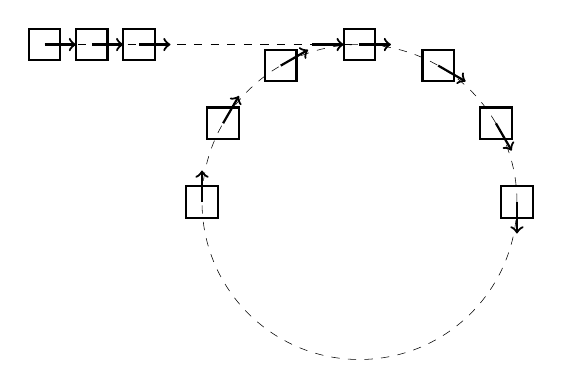
\begin{tikzpicture}[scale=2]
  % trace
  \draw[dashed, very thin] (-2cm, 1cm) -- (0, 1cm);
  \draw[dashed, very thin] (0,0) circle [radius=1cm];

  % leading nodes
  \foreach \x in {-2, -1.7, ..., -1.4} {
    \draw[thick] (\x cm, 1cm) +(-0.1, -0.1) rectangle ++(0.1, 0.1);
    \draw[thick, ->] (\x cm, 1cm) -- +(0.2, 0);
  }

  % cricular starting points
  \draw[thick, ->] (-0.3cm, 1cm) -- (-0.1cm, 1cm);

  % circular nodes
  \foreach \deg/\rot in {90/0, 60/-30, 30/-60, 0/-90, 180/90, 150/60, 120/30} {
    \draw[thick] (\deg : 1cm) +(-0.1, -0.1) rectangle ++(0.1, 0.1);
    \draw[thick, ->] (\deg : 1cm) -- +(\rot : 0.2);
  }
\end{tikzpicture}
\caption{A circular linked-list}
\label{fig:circular-list}
\end{figure}

\item In imperative settings, a linked-list may be corrupted, that it is circular. In such list, some node
points back to previous one. Figure \ref{fig:circular-list} shows such situation.
The normal iteration ends up infinite looping.
  \begin{enumerate}
    \item Write a program to detect if a linked-list is circular;
    \item Write a program to find the node where the loop starts (the node being pointed by two precedents).
  \end{enumerate}

\end{itemize}

\end{Exercise}

% ================================================================
%                 Appendix
% ================================================================

\begin{thebibliography}{99}

\bibitem{fp-pearls}
Richard Bird. ``Pearls of Functional Algorithm Design''. Cambridge University Press; 1 edition (November 1, 2010). ISBN: 978-0521513388

\bibitem{slpj-book-1987}
Simon L. Peyton Jones. ``The Implementation of Functional Programming Languages''. Prentice-Hall International Series in Computer Since. Prentice Hall (May 1987). ISBN: 978-0134533339

\bibitem{moderncxx}
Andrei Alexandrescu. ``Modern C++ design: Generic Programming and Design Patterns Applied''. Addison Wesley February 01, 2001, ISBN 0-201-70431-5

\bibitem{mittype}
Benjamin C. Pierce. ``Types and Programming Languages''. The MIT Press, 2002. ISBN:0262162091

\bibitem{unplugged}
Xinyu LIU. ``Isomorphism -- mathematics of programming''. 2020. \url{https://github.com/liuxinyu95/unplugged}

\bibitem{SICP}
Harold Abelson, Gerald Jay Sussman, Julie Sussman. ``Structure and Interpretation of Computer Programs, 2nd Edition''. MIT Press, 1996, ISBN 0-262-51087-1

\bibitem{okasaki-book}
Chris Okasaki. ``Purely Functional Data Structures''. Cambridge university press, (July 1, 1999), ISBN-13: 978-0521663502

\bibitem{algo-fp}
Fethi Rabhi, Guy Lapalme. ``Algorithms: a functional programming approach''. Second edition. Addison-Wesley, 1999. ISBN: 0201-59604-0

\bibitem{learn-haskell}
Miran Lipovaca. ``Learn You a Haskell for Great Good! A Beginner's Guide''. No Starch Press; 1 edition April 2011, 400 pp. ISBN: 978-1-59327-283-8

\bibitem{erlang}
Joe Armstrong. ``Programming Erlang: Software for a Concurrent World''. Pragmatic Bookshelf; 1 edition (July 18, 2007). ISBN-13: 978-1934356005

\bibitem{wiki-tail-call}
Wikipedia. ``Tail call''. https://en.wikipedia.org/wiki/Tail\_call

\bibitem{sgi-stl-transform}
SGI. ``transform''. http://www.sgi.com/tech/stl/transform.html

\bibitem{poj-drunk-jailer}
ACM/ICPC. ``The drunk jailer.'' Peking University judge online for ACM/ICPC. http://poj.org/problem?id=1218.

\bibitem{Haskell-wiki}
Haskell wiki. ``Haskell programming tips''. 4.4 Choose the appropriate fold. http://www.haskell.org/haskellwiki/Haskell\_programming\_tips

\bibitem{wiki-dot-product}
Wikipedia. ``Dot product''. http://en.wikipedia.org/wiki/Dot\_product

\end{thebibliography}

\ifx\wholebook\relax \else
\end{document}
\fi
